\documentclass[../main.tex]{subfiles}
\LoadClass[a4paper,12pt]{article}
\documentclass{article}

%%%%%%%%%%%%%%%%%%%%%%%%%%%%%%%
%     import des packages     %
%%%%%%%%%%%%%%%%%%%%%%%%%%%%%%%
\usepackage[export]{adjustbox}
\usepackage{algorithm}
\usepackage{algorithmic}
\usepackage{amsmath,amsfonts,amssymb}
\usepackage{anyfontsize}
\usepackage{array}
\usepackage[english]{babel}
\usepackage{colortbl}
\usepackage{comment}
\usepackage{cclicenses}
\usepackage{eqnarray}
\usepackage{eso-pic}
\usepackage{dirtree}
\usepackage{fancybox}
\usepackage{fancyhdr}
\usepackage{float}
\usepackage[T1]{fontenc} 
\usepackage{forest}
\usepackage{fourier-orns}
\usepackage{gensymb}
\usepackage{geometry}
\usepackage{glossaries}
\usepackage{graphicx}
\usepackage{hyperref}
\usepackage{ifthen}
\usepackage{import}
\usepackage{indentfirst}
\usepackage[utf8]{inputenc}
\usepackage{lastpage}
\usepackage{libertine}
\usepackage{lipsum}
\usepackage{listings}
\usepackage{mathtools}
\usepackage{mdframed}
\usepackage{multicol}
\usepackage{pdfpages}
\usepackage{pifont}
\usepackage{stmaryrd}
\usepackage{subcaption}
\usepackage{subfiles}
\usepackage{tabularx}
% \usepackage{tcolorbox}
\usepackage[most]{tcolorbox}
\usepackage{textcomp}
\usepackage{ulem}
\usepackage{wrapfig}

%%%%%%%%%%%%%%%%%%%%%%%%%%%%%%%%%%%%%%%%%%%%%%%%%%%%%%%%%
%    Renseigner les titres et variables importantes     %
%%%%%%%%%%%%%%%%%%%%%%%%%%%%%%%%%%%%%%%%%%%%%%%%%%%%%%%%%
\newcommand{\titre}{Multi-robot coordination}
\newcommand{\soustitre}{Autonomous exploration of gallery networks}
\newcommand{\sujet}{Engineering Graduation Project}
\newcommand{\sujets}{Seatech 3A - MOCA}
\newcommand{\auteur}{Fabien MATHÉ}
\newcommand{\referent}{M. Mehmet ERSOY}
\newcommand{\reportdate}{\date}

\newcommand{\partA}{State of the art}
\newcommand{\partB}{Partie 2}
\newcommand{\partC}{Partie 3}
\newcommand{\partD}{Partie 4}
\newcommand{\partE}{Partie 5}

%%%%%%%%%%%%%%%%%%%
%     BOOLEEN     %
%%%%%%%%%%%%%%%%%%%

% Création des boolean
\newboolean{abst}
\newboolean{thx}
\newboolean{contents}
\newboolean{introduction}
\newboolean{pt2}
\newboolean{pt3}
\newboolean{pt4}
\newboolean{pt5}
\newboolean{conclusion}
\newboolean{perspectives}
\newboolean{glossaire}
\newboolean{biblio}
\newboolean{annexe}


% Renseigner si le Rapport contient un abstract
\setboolean{abst}{true}
% Renseigner si le Rapport contient des remerciements
\setboolean{thx}{true}
% Renseigner si le Rapport contient une table des matières
\setboolean{contents}{true}
% Renseigner si le Rapport contient une introduction
\setboolean{introduction}{true}
% Renseigner si le Rapport contient une partie 2
\setboolean{pt2}{true}
% Renseigner si le Rapport contient une partie 3
\setboolean{pt3}{true}
% Renseigner si le Rapport contient une partie 4
\setboolean{pt4}{true}
% Renseigner si le Rapport contient une partie 5
\setboolean{pt5}{true}
% Renseigner si le Rapport contient une introduction
\setboolean{conclusion}{true}
% Renseigner si le Rapport contient des perspectives
\setboolean{perspectives}{true}
% Renseigner si le document contient une bibliographie
\setboolean{biblio}{true} 
% Renseigner si le document contient un glossaire
\setboolean{glossaire}{false}
% Renseigner si le Rapport contient des annexes 
\setboolean{annexe}{true}


%%%%%%%%%%%%%%%%%%%%%%%%%%%%%%%%%%%%%%
%     En-têtes en pieds de pages     %
%%%%%%%%%%%%%%%%%%%%%%%%%%%%%%%%%%%%%%
\geometry{hmargin=2cm,vmargin=2.3cm}
\pagestyle{fancy}
\fancyhfoffset[]{0pt}
\setlength{\headheight}{28pt}
\lhead{
\includegraphics[height = 0.6cm]{IMAGES/logos/Logo_SeaTech_2023.png}}
% \rhead{
\includegraphics[height = 0.7cm]{IMAGES/logos/MOCA.png}}
\rhead{\textsc{\leftmark}}

% Update \rightmark with \section name
\renewcommand{\sectionmark}[1]{\markboth{#1}{#1}}


\lfoot{\auteur}
\cfoot{ }
\rfoot{Page \thepage \ / \pageref{LastPage}}

\title{\titre}
\author{\auteur}
\date{\today}

%%%%%%%%%%%%%%%%%%%%%%%%%%%%%%
%     Autre mise en page     %
%%%%%%%%%%%%%%%%%%%%%%%%%%%%%%
\numberwithin{figure}{section}
\numberwithin{table}{section}

\setcounter{tocdepth}{2} % Change to 1 to exclude subsections as well


\newcommand{\citeURL}[1]{\href{#1}{\detokenize{#1}}}

% Création du compteur d'annexes
\newcounter{annexecounter}

% Définition de la commande pour les annexes
\NewDocumentCommand{\annexe}{m}{%
    \stepcounter{annexecounter} % Incrémenter le compteur d'annexes
    \subsection*{Annexe \arabic{annexecounter} - #1} % Affichage du texte avec le numéro et le titre
	\label{sec:#1}
}

\newcommand{\tobedone}{\textcolor{red}{\LARGE \textbf{TO BE DONE}}}
\newcommand{\annexetonum}{\textcolor{red}{\LARGE \textbf{ANNEXE ...}}}

\renewcommand{\familydefault}{\sfdefault}



%%%%%%%%%%%%%%%%%%%%%%%%%%%%%%%%%
%     Mise en page des codes    %
%%%%%%%%%%%%%%%%%%%%%%%%%%%%%%%%%
\definecolor{codegreen}{rgb}{0,0.6,0}
\definecolor{codegray}{rgb}{0.5,0.5,0.5}
\definecolor{codepurple}{rgb}{0.58,0,0.82}
\definecolor{backcolour}{rgb}{0.95,0.95,0.92}

\lstdefinestyle{python}{
	backgroundcolor=\color{backcolour},
	commentstyle=\color{codegreen},
	keywordstyle=\color{blue},
	numberstyle=\tiny\color{codegray},
	stringstyle=\color{codepurple},
	basicstyle=\ttfamily\scriptsize,
	breakatwhitespace=false,
	breaklines=true,
	captionpos=b,
	keepspaces=true,
	numbers=left,
	numbersep=5pt,
	showspaces=false,
	showstringspaces=false,
	showtabs=false,
	tabsize=2
}

\lstset{style=python}
\definecolor{codegreen}{rgb}{0,0.6,0}
\definecolor{codegray}{rgb}{0.5,0.5,0.5}
\definecolor{codepurple}{rgb}{0.58,0,0.82}
\definecolor{backcolour}{rgb}{0.95,0.95,0.92}

\lstdefinestyle{cpp}{
	backgroundcolor=\color{backcolour},
	commentstyle=\color{codegreen},
	keywordstyle=\color{blue},
	numberstyle=\tiny\color{codegray},
	stringstyle=\color{codepurple},
	basicstyle=\ttfamily\scriptsize,
	breakatwhitespace=false,
	breaklines=true,
	captionpos=b,
	keepspaces=true,
	numbers=left,
	numbersep=5pt,
	showspaces=false,
	showstringspaces=false,
	showtabs=false,
	tabsize=2,
	language=C++
}

\lstset{style=cpp}

\definecolor{codegreen}{rgb}{0,0.6,0}
\definecolor{codegray}{rgb}{0.5,0.5,0.5}
\definecolor{codepurple}{rgb}{0.58,0,0.82}
\definecolor{backcolour}{rgb}{0.95,0.95,0.92}

\lstdefinestyle{fortran}{
    backgroundcolor=\color{backcolour},
    commentstyle=\color{codegreen},
    keywordstyle=\color{blue},
    numberstyle=\tiny\color{codegray},
    stringstyle=\color{codepurple},
    basicstyle=\ttfamily\scriptsize,
    breakatwhitespace=false,
    breaklines=true,
    captionpos=b,
    keepspaces=true,
    numbers=left,
    numbersep=5pt,
    showspaces=false,
    showstringspaces=false,
    showtabs=false,
    tabsize=2,
    language=[90]Fortran
}

\lstset{style=fortran}


%%%%%%%%%%%%%%%%%%%%%%%%%%%%%%%%%%%%%%%%%%%%%%%%%%%%%%%%%%%%%%%%%%%%%%%%%%%%%%%%%%%%%%%%%%%%%%%%%%%%%%%%%%%%%%%%%%%%%%%
%                                                  Début du document                                                  %
%%%%%%%%%%%%%%%%%%%%%%%%%%%%%%%%%%%%%%%%%%%%%%%%%%%%%%%%%%%%%%%%%%%%%%%%%%%%%%%%%%%%%%%%%%%%%%%%%%%%%%%%%%%%%%%%%%%%%%%

\begin{document}

%%%%%%%%%%%%%%%%%%%%%%%%%
%     Page de garde     %
%%%%%%%%%%%%%%%%%%%%%%%%%
\begin{titlepage}
	\AddToShipoutPictureBG*{
\includegraphics[width=\paperwidth,height=\paperheight]{IMAGES/PageDeGardeRapport.png}}
	\begin{figure}[H]
		\begin{subfigure}{0.45\linewidth}
				
\includegraphics[width=0.6\textwidth,left]{IMAGES/logos/Logo_SeaTech_2023.png}
		\end{subfigure}
		\hfill
		\begin{subfigure}{0.45\linewidth}
				% 
\includegraphics[width=0.6\textwidth,right]{IMAGES/logos/MOCA.png}
		\end{subfigure}
	\end{figure}

	\centering

	% Espacement vertical
	\vspace*{5cm}

	% Barres horizontales
	\makebox[0.7\linewidth]{\hrulefill}\\[0.2cm]

	% Titre encadré
	\vspace{0.5cm}
	\begin{minipage}{\textwidth}
		\centering
		{\fontsize{28}{48}\selectfont \textsc{\titre}}\\[0.2cm]

		{\fontsize{18}{48}\selectfont \textsc{\soustitre}}
	\end{minipage}
	\vspace{0.3cm}

	% Barres horizontales
	\makebox[0.8\linewidth]{\hrulefill}\\[0.2cm]

	% Espacement vertical
	\vspace{3cm}

	% Description
		\large{\Large \textbf{\sujet}}\\
		\large{\textbf{\sujets}}\\

		\vspace{0.5cm}
		\large{\textbf{\reportdate}}

	\vspace{2cm}

	\begin{minipage}{0.20\textwidth}

	\end{minipage}
	\hfill
	\begin{minipage}{0.35\textwidth}
		\begin{flushleft}
			Auteur : \\
			\auteur
		\end{flushleft}
	\end{minipage}
	\begin{minipage}{0.09\textwidth}
		% Section vide pour espacement optimal
	\end{minipage}
	\hfill
 	\begin{minipage}{0.3\textwidth}
		\begin{flushleft}
			Enseignant : \\
			\referent

		\end{flushleft}
	\end{minipage}


\end{titlepage}

\ClearShipoutPictureBG

\newpage

\renewcommand{\thepage}{}

\renewcommand{\thepage}{\arabic{page}}
\renewcommand{\thesection}{\Roman{section}}

%%%%%%%%%%%%%%%%%%
%     Résumé     %
%%%%%%%%%%%%%%%%%%
\ifthenelse{\boolean{abst}}{
	\addcontentsline{toc}{section}{\protect\numberline{}Résumé}%
	\subfile{SECTIONS/1resume}

	\newpage
}

%%%%%%%%%%%%%%%%%%%%%%%%%
%     Remerciements     %
%%%%%%%%%%%%%%%%%%%%%%%%%
\ifthenelse{\boolean{thx}}{
	\addcontentsline{toc}{section}{\protect\numberline{}Remerciements}%
	\subfile{SECTIONS/2remerciements}

	\newpage
}

%%%%%%%%%%%%%%%%%%%%%%%%%%%%
%     Plan du document     %
%%%%%%%%%%%%%%%%%%%%%%%%%%%%

\ifthenelse{\boolean{contents}}{
	\vfill
	\tableofcontents
	\vfill
	
	\newpage
}

%%%%%%%%%%%%%%%%%%%%%%%%
%     INTRODUCTION     %
%%%%%%%%%%%%%%%%%%%%%%%%
\ifthenelse{\boolean{introduction}}
{
	\addcontentsline{toc}{section}{\protect\numberline{}Introduction}%
	\section*{Introduction}

	\markboth{Introduction}{Introduction} % Manually update \rightmark for section*
	\subfile{SECTIONS/3introduction}


	\newpage
}


%%% PARTIE 1 %%%
\section{\partA}
\subfile{SECTIONS/part1}

%%% PARTIE 2 %%%
\newpage
\ifthenelse{\boolean{pt2}}
{
	\section{\partB}
	\subfile{SECTIONS/part2}
	
	\newpage
}
	
	
%%% PARTIE 3 %%%
\ifthenelse{\boolean{pt3}}
{
	\section{\partC}
	\subfile{SECTIONS/part3}
	
	\newpage
}
	
	
%%% PARTIE 4 %%%
\ifthenelse{\boolean{pt4}}
{
	\section{\partD}
	\subfile{SECTIONS/part4}
	
	\newpage
}
	
%%% PARTIE 5 %%%
\ifthenelse{\boolean{pt5}}{
	\section{\partE}
	\subfile{SECTIONS/part5}

	\newpage
}
		
%%%%%%%%%%%%%%%%%%%%%%
%     CONCLUSION     %
%%%%%%%%%%%%%%%%%%%%%%
\ifthenelse{\boolean{perspectives}}
{
	\addcontentsline{toc}{section}{\protect\numberline{}Conclusion}%
	\section*{Conclusion}
	\markboth{Introduction}{Introduction} % Manually update \rightmark for section*

	\subfile{SECTIONS/Wconclusion}

	\newpage
}



\ifthenelse{\boolean{perspectives}}
{
	\section*{Perspectives}
	\addcontentsline{toc}{section}{\protect\numberline{}Perspectives}
	\subfile{SECTIONS/Xperspectives}
	
	\newpage 
}

%%%%%%%%%%%%%%%%%%%%%%%%%
%     Bibliographie     %
%%%%%%%%%%%%%%%%%%%%%%%%%

\ifthenelse{\boolean{biblio}}
{
	\addcontentsline{toc}{section}{\protect\numberline{}References}
	% \bibliographystyle{unsrt}
	\bibliographystyle{IEEEtran}
	\footnotesize{\bibliography{BIBLIOGRAPHY/bib.bib}}

	\newpage
}


%%%%%%%%%%%%%%%%%%%%%
%     Glossaire     %
%%%%%%%%%%%%%%%%%%%%%
\normalsize
\ifthenelse{\boolean{glossaire}}
{
	\section*{Glossaire}
	\makeglossaries
	\printglossaries
	\addcontentsline{toc}{section}{\protect\numberline{}Glossaire}%
	\subfile{SECTIONS/Yglossaire}
	
	\newpage
}

%%%%%%%%%%%%%%%%%%%
%     Annexes     %
%%%%%%%%%%%%%%%%%%%
\ifthenelse{\boolean{annexe}}
{
	\section*{Annexes}
	\addcontentsline{toc}{section}{\protect\numberline{}Annexes}%
	\subfile{SECTIONS/Zannexes}
}


\end{document}


\begin{document}

\subsection{Global path theory}
In this section, we introduce the preliminary for mathematical optimization of the path. Several challenging problems arise, which are described at the end of this section.

we consider the theoretical path that the robot should follow in a space with obstacles, without taking into account the feasibility constraints imposed by the robot's physical limitations. This theoretical path is derived based on the shortest distance to the target while avoiding obstacles.

\vspace{1em}

Let $\Omega \in \mathbb{R}^{2}$ standing as the world, and let $\mathbf{X}(t)$ be the coordinates of the robot at time $t$ in this space.
\vspace{0.5em}
Let $FV(t)$ be the field of vision of the robot at time $t$.
\vspace{0.5em}

Let $\mathbf{M}(t, \theta)$ be the first intersection point between a segment and the walls,
\vspace{0.5em}

\begin{equation*}
	\displaystyle
	\mathbf{M}(t, \theta) = \mathbf{X}(t) + R(t, \theta) 
	\begin{pmatrix}
		\cos \theta & 0\\
		0 & \sin \theta\\
	\end{pmatrix} 
	\mathbf{X}(t)
\end{equation*}

We denote $\mathbf{M}_{max} (t, \theta)$ as the point such that $R(t, \theta) = R_{max}$.
\vspace{0.5em}

Here, $R$ is the minimale distance between the point and all the intersection points between a segment and the map
\begin{equation*}
	\displaystyle
	R(t, \theta) = 
	\begin{cases*}
		\min(\text{\rmfamily distance}( \, \mathbf{X}(t), \, P_i(t, \theta) \,)), \forall i \in \{0, \ldots, \text{\rmfamily Card}(P) - 1\} \text{\rmfamily if Card}(P) > 0,\\
		R_{max}, \text{\rmfamily otherwise}.
	\end{cases*}
\end{equation*}

% \begin{equation*}
% 	\displaystyle
% 	R(t, \theta) = 
% 	\begin{cases*}
% 		\min(\text{\rmfamily distance}( \, \mathbf{X}(t), \, P_i(t, \theta) \,)),& \forall i \in [[0, \text{\rmfamily Card}(P)]] \text{\rmfamily if Card}(P) > 0, \\
% 		R_{max} \text{\rmfamily otherwise}.
% 	\end{cases*}
% \end{equation*}

where $P(t, \theta) = \{L(t, \theta) \cap W\}$ is the set of all intersection point between the segment $L$ and the segment of the map and $Card(P)$ the number of element in this set

\begin{equation*}
	\displaystyle
	L(t, \theta) = \left\{ \, (1 - l) \, \mathbf{X}(t) + l\, \mathbf{M}_{max}(t, \theta) \,|\, l \in [0, 1]\, \right\}
\end{equation*}

\begin{equation*}
	\displaystyle
	W = \left\{ \, \text{\rmfamily Segment} (\Omega)\, \right\}
\end{equation*}

We define the field of vision of the robot as:

\begin{equation}
	\displaystyle
	FV(t) = \left\{ \, (1 - l) \, \mathbf{X}(t) + l\, \mathbf{M}(t, \theta) \,|\, l \in [0, 1], \theta \in [0, 2 \pi[ \, \right\}
\end{equation}

In other words, $FV(t)$ is the set of points in $\Omega$ present in a disk of radius $R_{max}$ and located between the robot and the nearest intersection with a wall.
\vspace{0.5em}

We now construct the functional that we will later seek to optimize, which is related to the movement of the robot.
\vspace{0.5em}

We define $\mathit{KM}$ (\textit{Known Map}) as the space of the map known by the robot and $\mathit{EM}$ (\textit{Explorable Map}) as the part of $\Omega$ explorable by the robot.
\begin{equation}
	\displaystyle
	J(\mathbf{X}(t)) = \int_{0}^{T} | \mathbf{\dot{X}}(t) | dt
\end{equation}
\vspace{0.5em}

$J$ is a functional function of the initial position of the robot, giving the length of the path traveled by the robot before $t = T$.
\vspace{0.5em}

$T$ is the time at which the map is explored to the maximum capacity of the robot, i.e., $KM = EM$.
\vspace{0.5em}

To determine if $KM = EM$, we calculate the contours of the known domain. If all contours are closed, then $KM \subset EM$. Additionally, if the measures of $KM$ and $EM$, namely their areas, are equal, then we can reasonably say that $KM = EM$.
\vspace{0.5em}

For simplicity in studying the functional, we slightly modify it.
\begin{equation}
	\displaystyle
	J(\mathbf{X}(t)) = \frac{1}{2} \int_{0}^{T} \mathbf{\dot{X}}(t)^{2} dt
\end{equation}

\subsection{Local path theory}

\subsubsection{First approach: mathematical approach}

In this section, we focus on determining the optimal commands for navigating to a local waypoint obstacle-free while adhering to the robot's constraints. 

Optimal in this context means using the least amount of energy to move from point A to point B. Considering the robot moves using DC motors, the power consumption is proportional to the voltage for rotation speed and the current for the torque applied to the wheel. Assuming the floor is completely flat and the torque is constant, the current remains the same. Therefore, the energy consumption is only related to the wheel speed. We define the energy spent for moving as:

as a reminder, $\omega_L$ and $\omega_R$ are the speed of the left and right wheel.

$$
\displaystyle E(T) = \int_{0}^{T} \| \omega(t) \| \, dt
$$

with $\displaystyle \| \omega (t) \| = \sqrt{\omega_L^{2}(t) + \omega_R^{2}(t)}$ and  $\omega_{L, R} \,:\, \mathbb{R}_+ \longrightarrow [-\omega_{max}, \omega_{max}]$ 

Two constraint remains, we want $X(0) = X_R$ and $X(T) = X_{WP}$

In the part \figtonum, we calculated $\dot{X} = F(\omega)$.

Note:
If the current were not constant, we would need to account for the terrain characteristics and define the energy consumption as the product of voltage and current. In that case, $E(T)$ would become $\tilde{E}(T) = \int_{0}^{T} \| U(t) I(t) \| dt$, where $U(t)$ and $I(t)$ are functions dependent on the map characteristics. This would significantly complicate the problem. 


\subsubsection{Second approach: empirical approach}

This second approach consists of determining the set of all possible maximal paths achieved by the robot in a certain amount of time. Reversing the problem should give us the optimal commands to reach the waypoint.
In the first attempt, I focus on finding the maximal path using stochastic methods. Subsequently, I compute all possible combinations of paths with a given number of different commands.



\subsection{Introducing a new method for dynamic pathfinding}

In this section, we introduce a new method for real-time dynamic pathfinding. This method involves inflating the path perpendicular to the shortest path to a point, i.e., a line. The line is split if it is not free from obstacles within a given safe range.

For our study, it is crucial that this algorithm runs in real-time to avoid any obstacles. Since the goal is to explore a map using multiple robots, we must ensure that the path computation time for each robot is minimal so that they can avoid each other.  

The principle is simple: draw a straight line between the robot and the waypoint (\autoref{fig:draw_line}). If the path is not free of obstacles within the defined safe range (\autoref{fig:check_line}), split the path in the middle and shoot points perpendicular to the line (\autoref{fig:shoot_line}). When a shot point is free from obstacles, validate the point and check if the two resulting lines are free from obstacles (\autoref{fig:validate_point}). If not, repeat the steps described above on the new lines (\autoref{fig:repeat_method}). Once all points are safe, simplify the path using a straightforward algorithm. The process can be visualized on \autoref{fig:method_visu}.

\begin{figure}[H]
	\centering
	\begin{subfigure}[b]{0.45\textwidth}
		\centering
		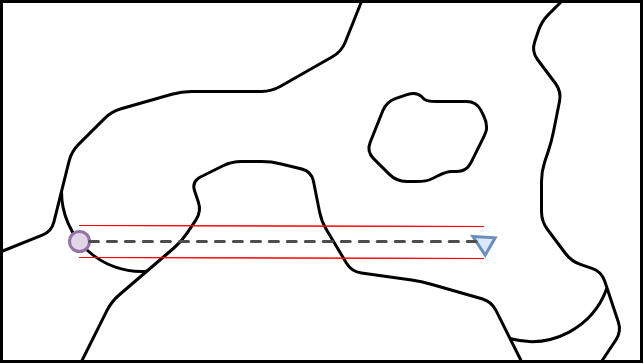
\includegraphics[width=\textwidth]{IMAGES/part3/methode1.png}
		\caption{Draw a straight line with safe range}
		\label{fig:draw_line}
	\end{subfigure}
	\hfill
	\begin{subfigure}[b]{0.45\textwidth}
		\centering
		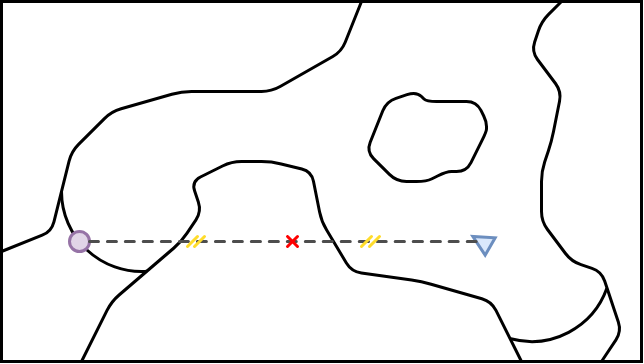
\includegraphics[width=\textwidth]{IMAGES/part3/methode2.png}
		\caption{Check if the path is free}
		\label{fig:check_line}
	\end{subfigure}
	\vfill
	\begin{subfigure}[b]{0.45\textwidth}
		\centering
		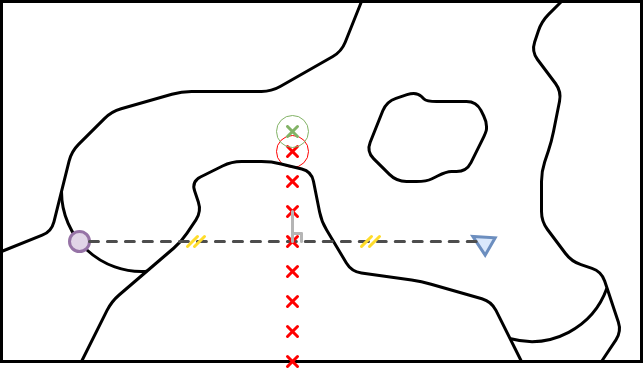
\includegraphics[width=\textwidth]{IMAGES/part3/methode3.png}
		\caption{Shoot points perpendicular}
		\label{fig:shoot_line}
	\end{subfigure}
	\hfill
	\begin{subfigure}[b]{0.45\textwidth}
		\centering
		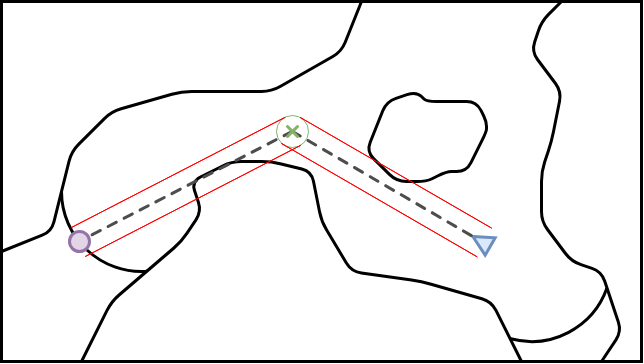
\includegraphics[width=\textwidth]{IMAGES/part3/methode4.png}
		\caption{Validate the point}
		\label{fig:validate_point}
	\end{subfigure}
	\vfill
	\begin{subfigure}[b]{0.45\textwidth}
		\centering
		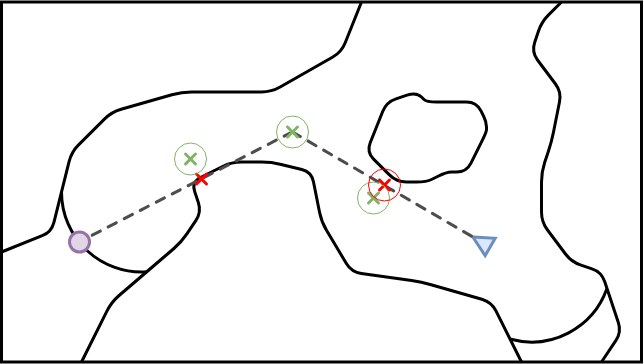
\includegraphics[width=\textwidth]{IMAGES/part3/methode5.png}
		\caption{Repeat the method}
		\label{fig:repeat_method}
	\end{subfigure}
	\hfill
	\begin{subfigure}[b]{0.45\textwidth}
		\centering
		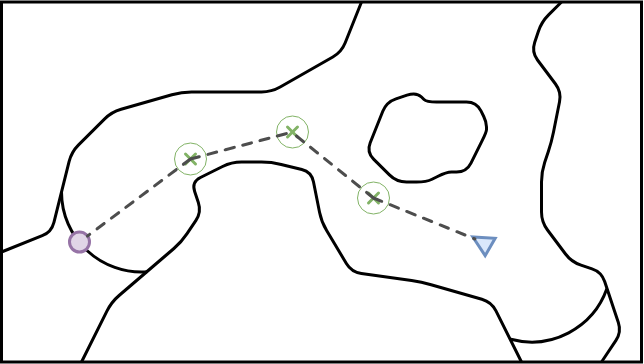
\includegraphics[width=\textwidth]{IMAGES/part3/methode6.png}
		\caption{Connect points}
		\label{fig:idk}
	\end{subfigure}
	\caption{Visualization of the dynamic pathfinding method}
	\label{fig:method_visu}
\end{figure}



\textbf{Path simplification}

The goal of this algorithm is to ensure that the path is the shortest possible by simplifying it. The algorithm iterates through all the points in the path. For each point, it checks if the path to the next point is obstacle-free. If it is, the algorithm continues to the next point. If the path is not free, the algorithm keeps the last valid point and starts the process again from there. This way, the path is simplified by removing unnecessary intermediate points while ensuring it remains obstacle-free. The method can be visualized on the \autoref{fig:path_simp}.

\begin{figure}[H]
	\centering
	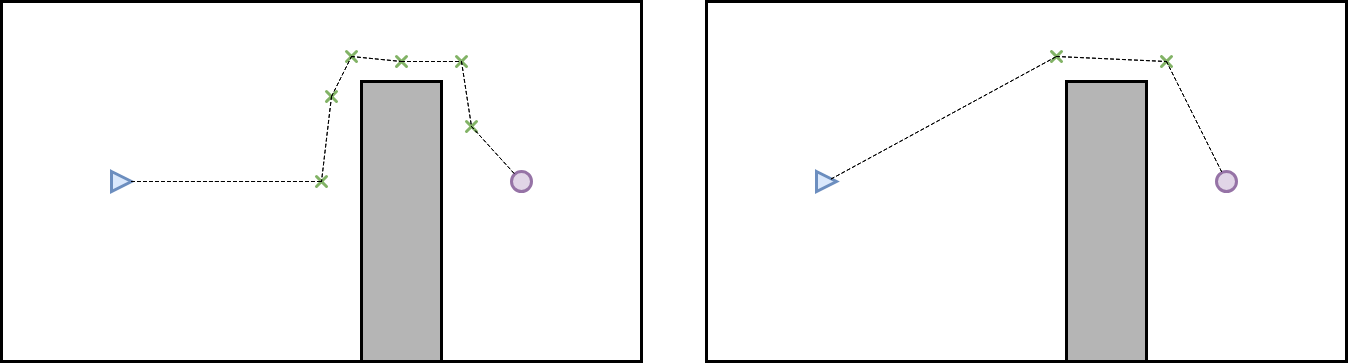
\includegraphics[width=0.9\textwidth]{IMAGES/part3/shorten_path.png}
	\caption{Path simplification process}
	\label{fig:path_simp}
\end{figure}

To ensure this algorithm works and to measure its performance, I conducted a small benchmark. While the benchmark can be theoretically calculated, I also explored a numerical method for computing the shortest path to handle various scenarios. The benchmark will serve as a performance estimator for the numerical method.

\subsection{Finding the shorthest path distance}
To find the shortest path, I like to take inspiration from nature by simulating a wave propagating through a medium. This way, the shortest path naturally emerges as the one the wave follows.  

\vspace{1em}

The wave equation describes how information spreads at a certain speed, but challenges arise—how to model refraction, how to ensure the wave propagates at a constant speed. To tackle this, I used a cellular automaton once again. Made for propagating information, they are an interesting tool for this approach.\cite{tapia_2016}

\vspace{1em}

Differently from the part \figtonum, I will use cellular automata as a computational tool for simulating phenomenon. Application were found in various domain from physics to biology. Lattice Gaz Cellular Automata (LGCA) for instance are used to simulate gaz fluid flows, it is the precursor of the lattice Boltzman Method (LBM)\cite{chen_1998}

\vspace{1em}

Based on the work of \textit{Calvo Tavia} and \textit{al.}\cite{tapia_2016}, the process is describe below:

\vspace{1em}

Given a lattice $\Lambda = \{(i,j) \in \mathbb{N}^{2} \,:\, 1 \leq i, j \leq L\}$ with $L$ the size of the lattice, we define the following sets:
\vspace{1em}

\begin{itemize}
	\item $A_t = \{ (i, j) \in \Lambda \,:\, a_t(i, j) > 0\}$: the set of activated cells at time $t$
	\item $\mathcal{B}$: the set of obstacles
	\item $\Gamma \subset \Lambda$: the set of secondary wave sources
	\item $E_t$: the set of empty spaces
	\item $\mathcal{M}_{ij} = \{ (k, l) \in \Lambda \,:\, \|(k - i, l - j)\|_{\infty} = 1\}$: the Moore neighborhood of a cell $(i, j)$
\end{itemize}

\vspace{1em}

Each cell of the lattice carries 2 variables:
\begin{itemize}
	\item $a_t (i, j)$: the state of the cell $(i, j)$ at time $t$
	\item $z_t (i, j)$: the distance vector of the wave from the source to the cell $(i, j)$ at time $t$, defined as:
	$z_t (i, j) = \begin{pmatrix}
		\text{Total number of steps taken to arrive at cell } (i, j) \\
		\text{Number of diagonal steps among them}
	\end{pmatrix}$
\end{itemize}


\vspace{1em}


To update $z_t$, we introduce the following variable that track the distance of the wave from the source to the cell $(i, j)$ at time $t$: 
$$r_{t_{ij}} (k, l) = \begin{cases}
	(0, 0) & \text{if } (i, j) \in {E}_{t} \text{ or } (k, l) \notin A_t\\
	z(k, l) + (1, \mathbbm{1}_{D_{ij}}(k, l)) & \text{otherwise}
\end{cases}$$

where $\mathbbm{1}_{D_{ij}}$ the diagonal function indicator, i.e. 1 if $(k, l)$ is a diagonal neighbor of $(i, j)$ and $0$ otherwise.

$$D_{ij} = {(k, l) \in \Lambda \,:\, |k - i||l - j| = 1} \subset M_{ij}$$

Note that $\| r_{t_{ij}} \|_2$ is the distance mesurement from the wave source to the cell $(i, j)$.

\vspace{1em}
Moreover, we define the set of cells in the Moore neighborhood that could be a source of activation for the cell $(i, j)$ at time $t$ as:
$$ W_t = \{(k, l) \in M_{ij} \,:\, t < a_t (k, l) + \| r_{t_{ij}} \|_2 \leq t+1\}$$

\vspace{1em}
Finally, we define the pair $(k, l)$ where the distance $\| r_{t_{ij}} \|_2$ is minimal if the set of potential source of activation for the cell $(i, j)$ at time $t$ is not empty, i.e. $W_t \neq \emptyset$.:
$$(i_t^{*}, j_t^{*}) = 
\begin{cases}
	argmin\{\| r_{t_{ij}} (k, l)\|_2 \,:\, (k, l) \in W_{t_{ij}}\} & \text{if }  W_t \neq \emptyset\\
	(i, j) & \text{otherwise}
\end{cases}
$$


\vspace{1em}
After defining all the sets and variables above, the wave propagation is governed by the following rules:

\vspace{1em}

At each iteration of time, we compute the two variables $a_t (i, j)$ and $z(i, j)$ for each cell $(i, j) \in \Lambda$ as follows:
$$a_t (i, j) = 
\begin{cases}
	t +1 & \text{if }  (i, j) \in \Gamma \text{ or } (M_{ij} \cap  A_t) \neq \emptyset\\
	a_t(i_t^{*}, j_t^{*}) & \text{otherwise}
\end{cases}
$$


$$z_t (i, j) = 
\begin{cases}
	z_t(i_, j) & \text{if } (i, j) \notin E_t \backslash \Gamma \text{ or } W_t = \emptyset\\
	r_t(i_t^{*}, j_t^{*}) & \text{otherwise}
\end{cases}
$$

This implementation does not allow to track the refraction of the waves, these are wrongly reflected by the obstacles. To prevent front breaking in wave propagation near obstacles, the concept of "additional secondary" wave sources is introduced, inspired by Huygens' principle, where selected cells on the obstacle boundary generate secondary waves. An algorithm determines these sources based on geometric conditions, ensuring correct wave propagation by maintaining the expected wavefront shape even when interacting with obstacles. This simple algorithm is describe in the work of \textit{Calvo Tavia} and \textit{al.}\cite{tapia_2016}. We will not go into the details of the algorithm here.


\subsection{Analysis of the new methode}

Now I have an numerical method for computing the shortest path length, we can focus on performance of the algorithm introduced. Despite this algorithm is simple and fast, making it suitable for implementation on a large number of small chips, they have some limitations that can be critical for certain cases. A small benchmark was conducted with the following results.


Eight maps were introduced in this benchmark, as shown in \autoref{fig:benchmark_maps}. The maps are 1200 by 700 metric units, with the robot starting at the triangle located at coordinates (100, 350) and the target point at (1100, 350).

\begin{figure}[H]
	\centering
	\begin{subfigure}[b]{0.24\textwidth}
		\centering
		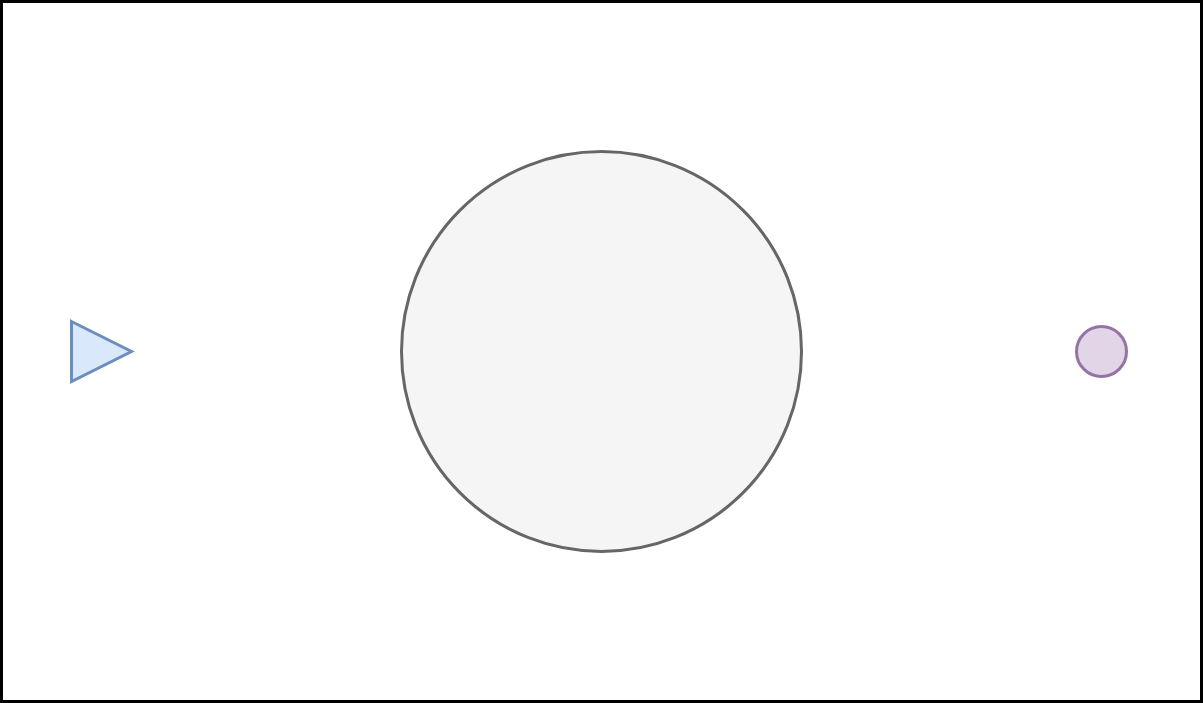
\includegraphics[width=\textwidth]{IMAGES/part3/map1.png}
		\caption*{Map 1}
		\label{fig:map1}
	\end{subfigure}
	\hfill
	\begin{subfigure}[b]{0.24\textwidth}
		\centering
		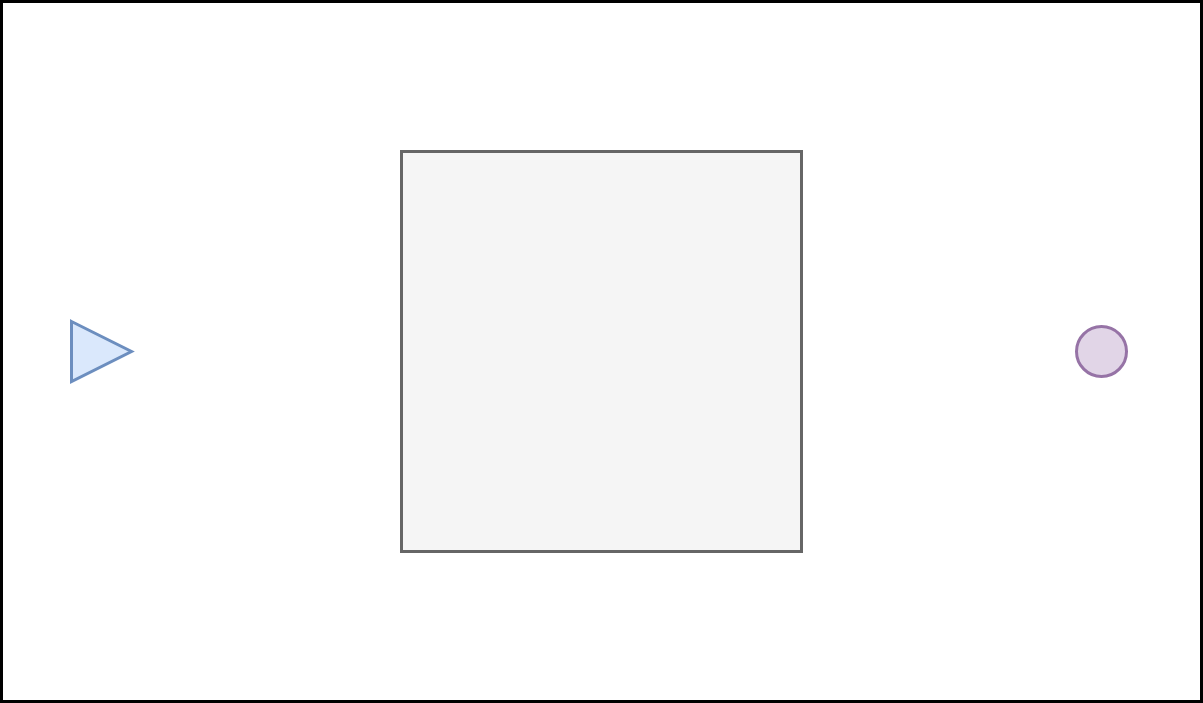
\includegraphics[width=\textwidth]{IMAGES/part3/map2.png}
		\caption*{Map 2}
		\label{fig:map2}
	\end{subfigure}
	\hfill
	\begin{subfigure}[b]{0.24\textwidth}
		\centering
		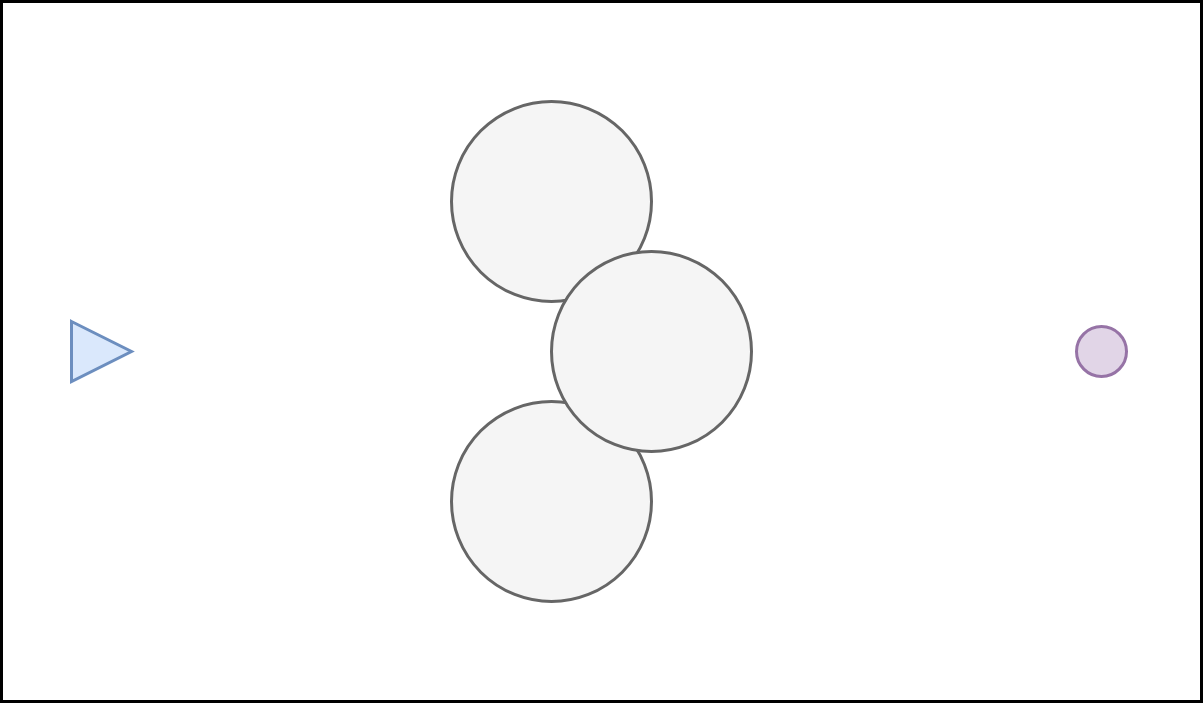
\includegraphics[width=\textwidth]{IMAGES/part3/map3.png}
		\caption*{Map 3}
		\label{fig:map3}
	\end{subfigure}
	\hfill
	\begin{subfigure}[b]{0.24\textwidth}
		\centering
		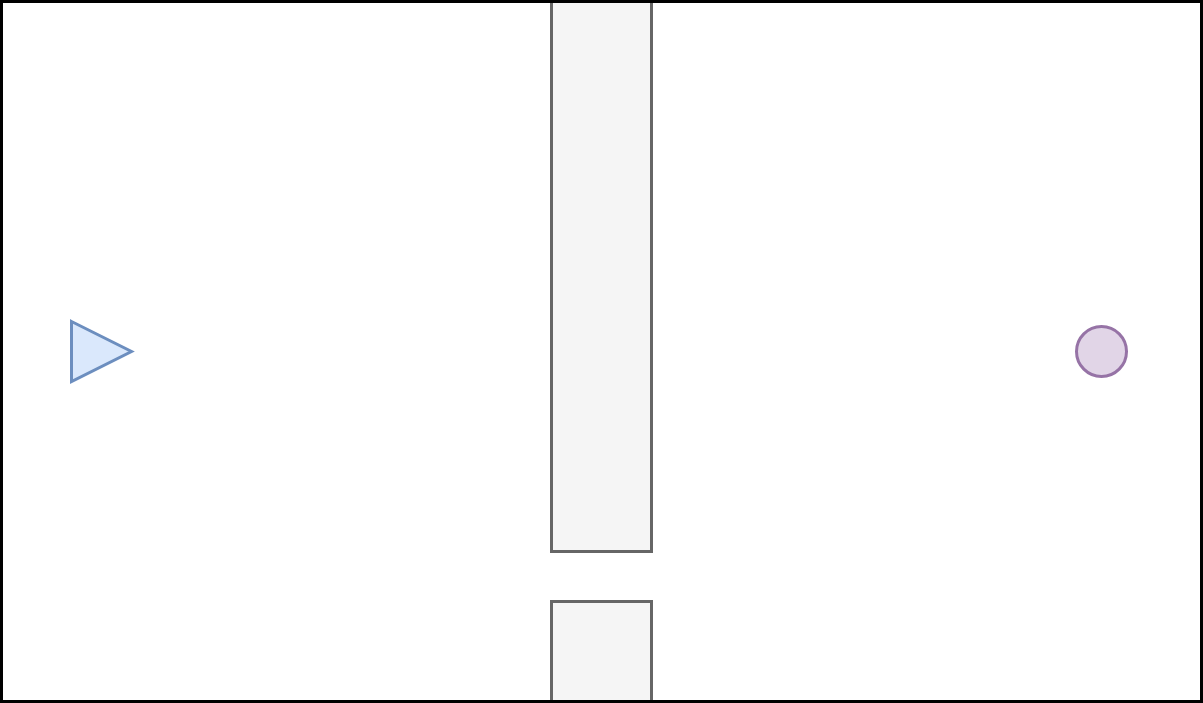
\includegraphics[width=\textwidth]{IMAGES/part3/map4.png}
		\caption*{Map 4}
		\label{fig:map4}
	\end{subfigure}
	\vfill
	\begin{subfigure}[b]{0.24\textwidth}
		\centering
		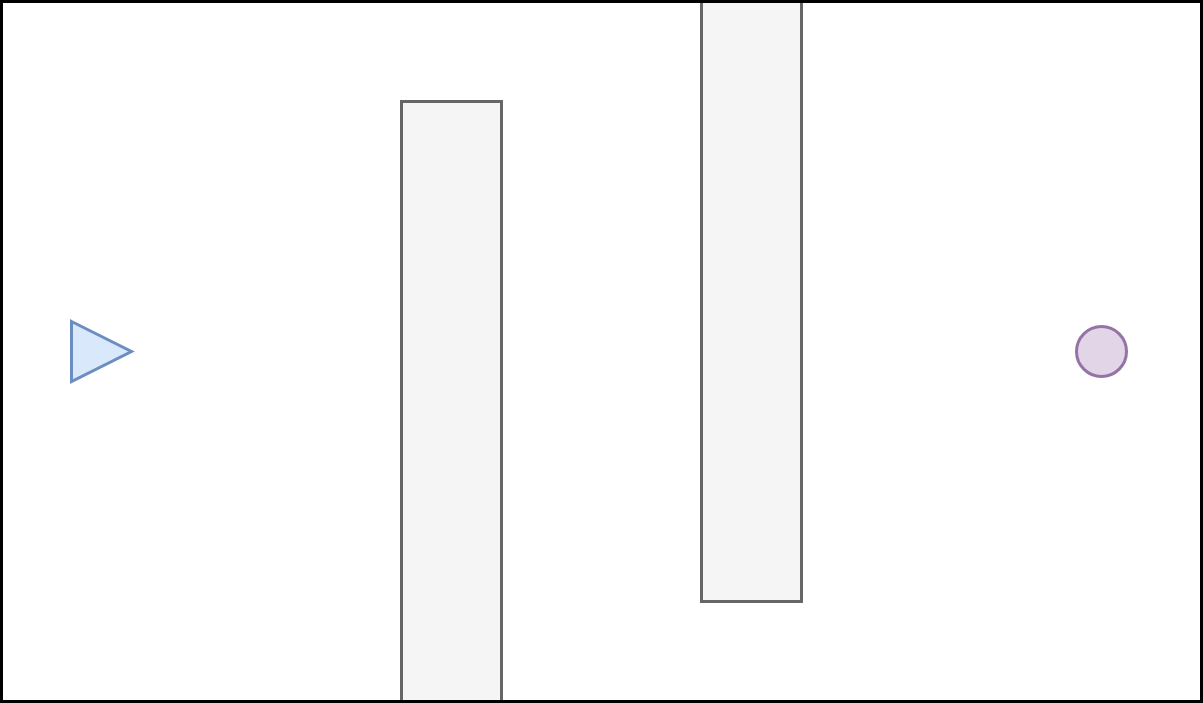
\includegraphics[width=\textwidth]{IMAGES/part3/map5.png}
		\caption*{Map 5}
		\label{fig:map5}
	\end{subfigure}
	\hfill
	\begin{subfigure}[b]{0.24\textwidth}
		\centering
		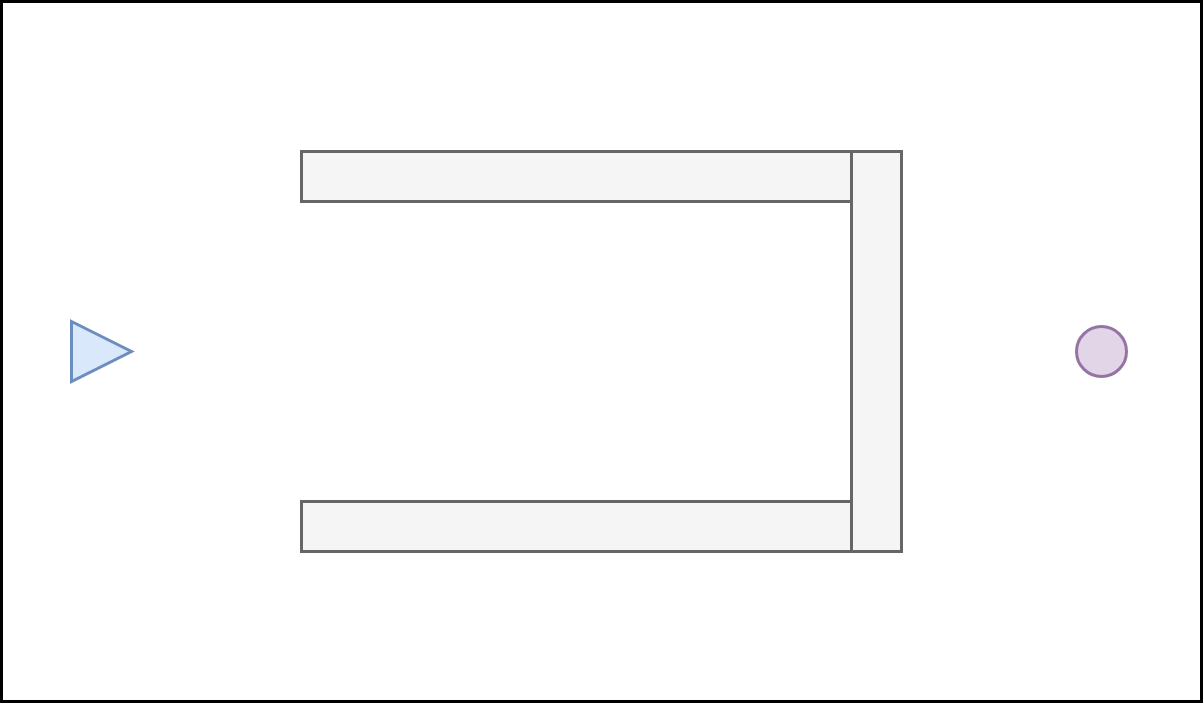
\includegraphics[width=\textwidth]{IMAGES/part3/map6.png}
		\caption*{Map 6}
		\label{fig:map6}
	\end{subfigure}
	\hfill
	\begin{subfigure}[b]{0.24\textwidth}
		\centering
		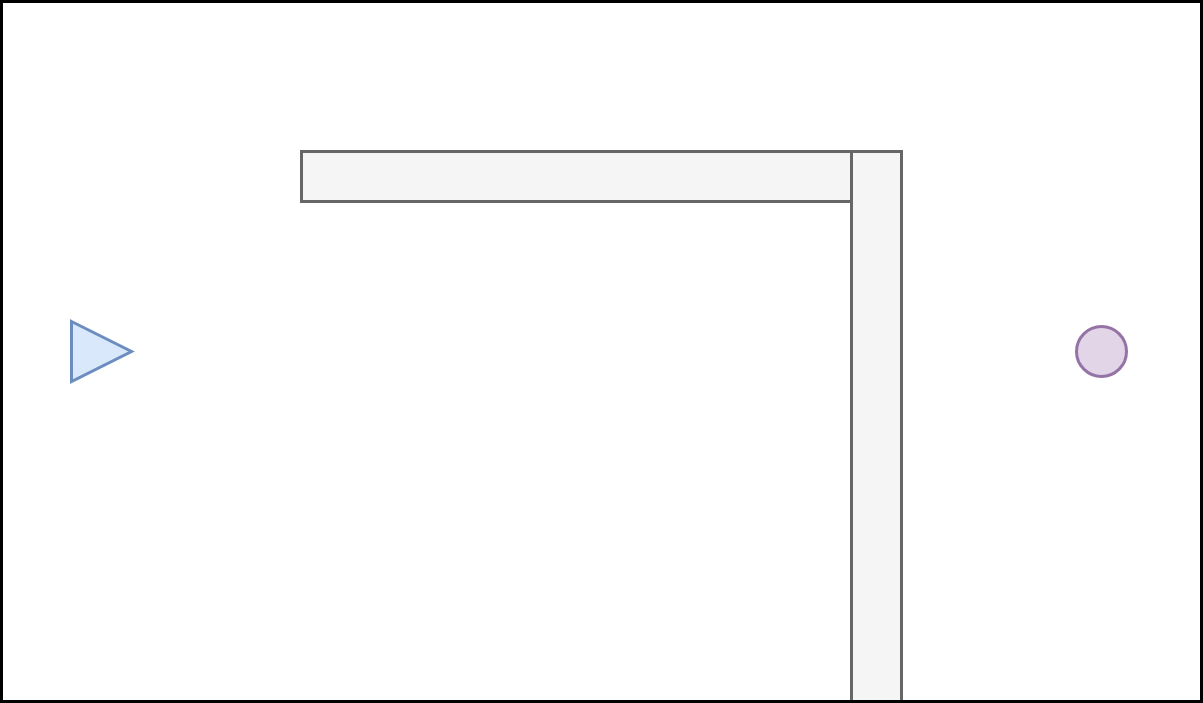
\includegraphics[width=\textwidth]{IMAGES/part3/map7.png}
		\caption*{Map 7}
		\label{fig:map7}
	\end{subfigure}
	\hfill
	\begin{subfigure}[b]{0.24\textwidth}
		\centering
		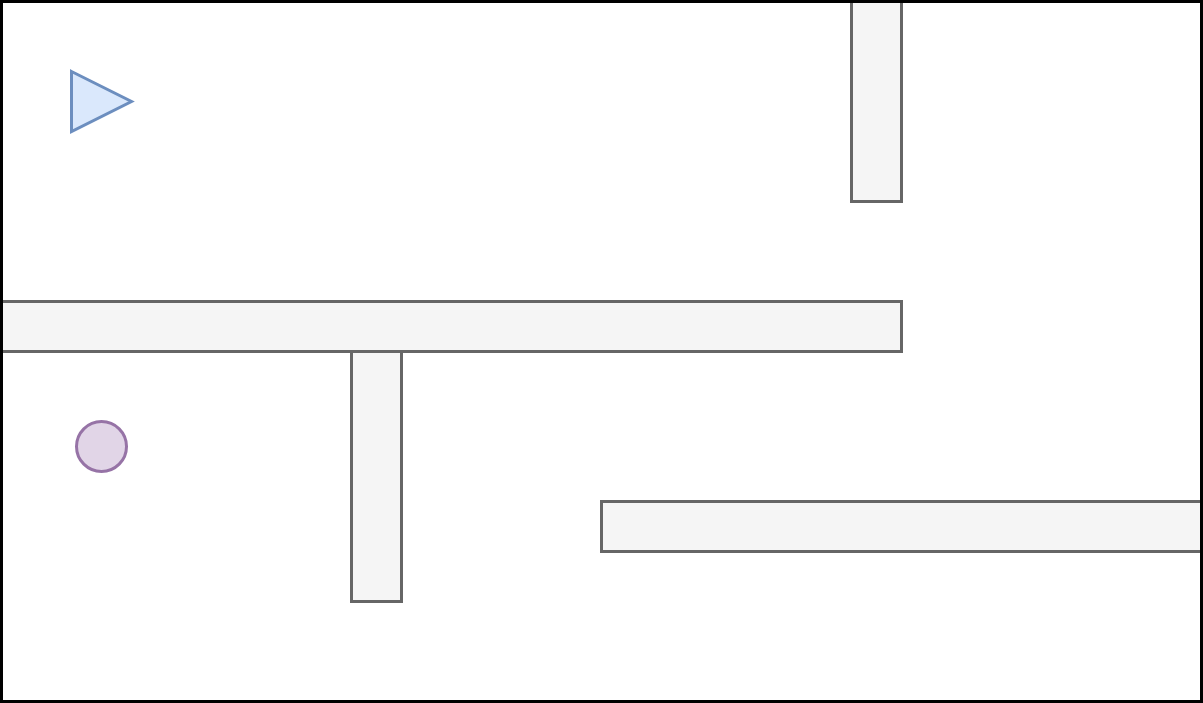
\includegraphics[width=\textwidth]{IMAGES/part3/map8.png}
		\caption*{Map 8}
		\label{fig:map8}
	\end{subfigure}
	\caption{Benchmark maps}
	\label{fig:benchmark_maps}
\end{figure}

\textbf{Results}
\begin{figure}[H]
	\centering
	\begin{subfigure}[b]{0.24\textwidth}
		\centering
		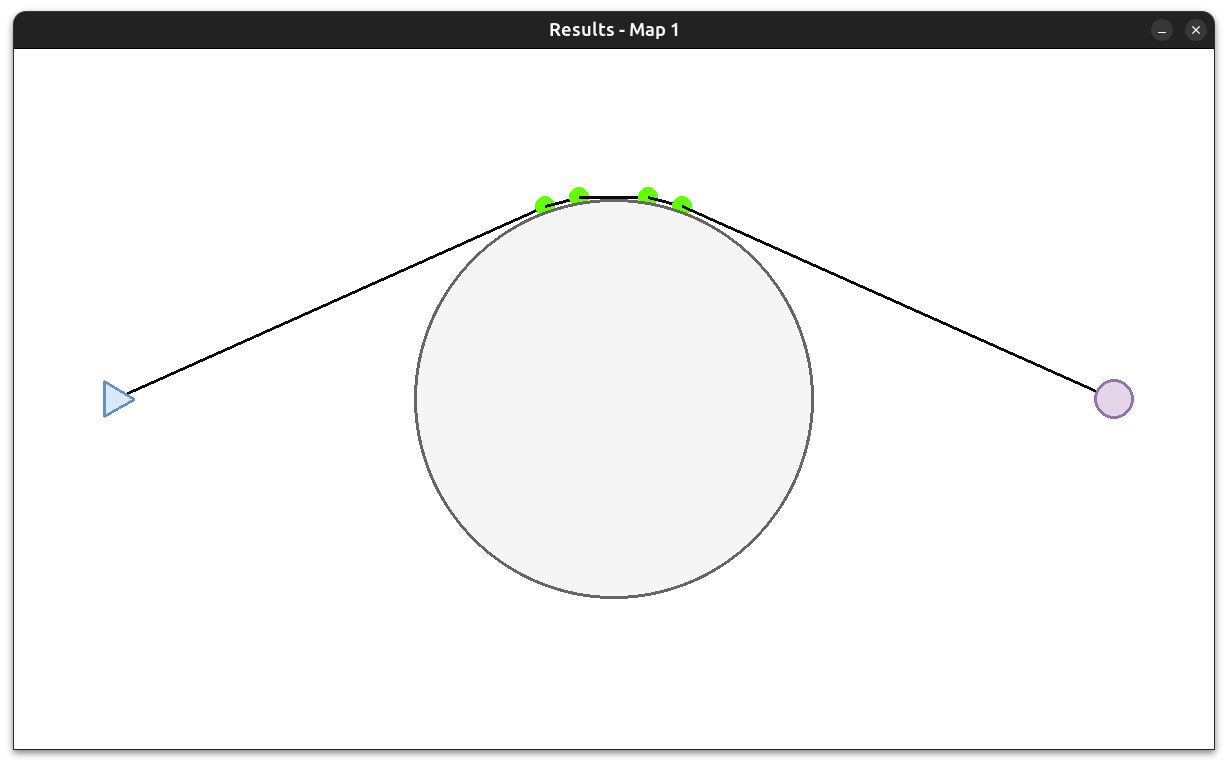
\includegraphics[width=\textwidth]{IMAGES/part3/rmap1.png}
		\caption*{Result for map 1}
		\label{fig:rmap1}
	\end{subfigure}
	\hfill
	\begin{subfigure}[b]{0.24\textwidth}
		\centering
		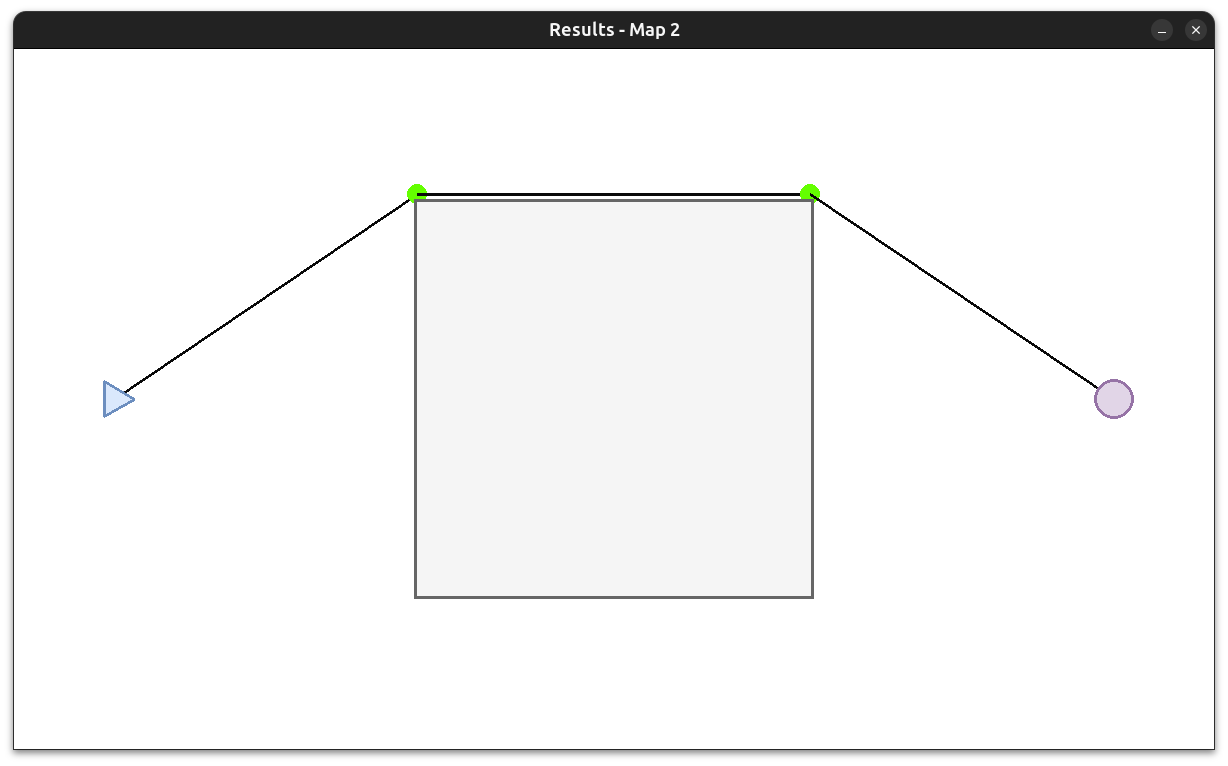
\includegraphics[width=\textwidth]{IMAGES/part3/rmap2.png}
		\caption*{Result for map 2}
		\label{fig:rmap2}
	\end{subfigure}
	\hfill
	\begin{subfigure}[b]{0.24\textwidth}
		\centering
		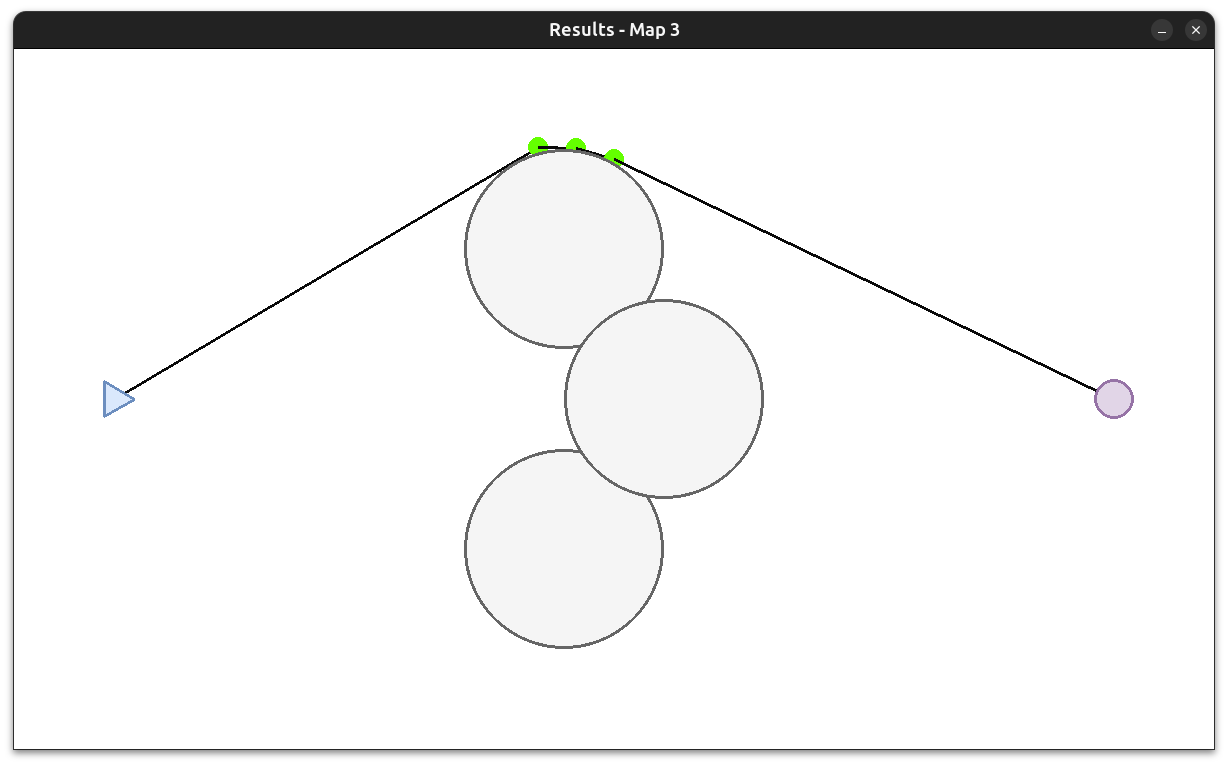
\includegraphics[width=\textwidth]{IMAGES/part3/rmap3.png}
		\caption*{Result for map 3}
		\label{fig:rmap3}
	\end{subfigure}
	\hfill
	\begin{subfigure}[b]{0.24\textwidth}
		\centering
		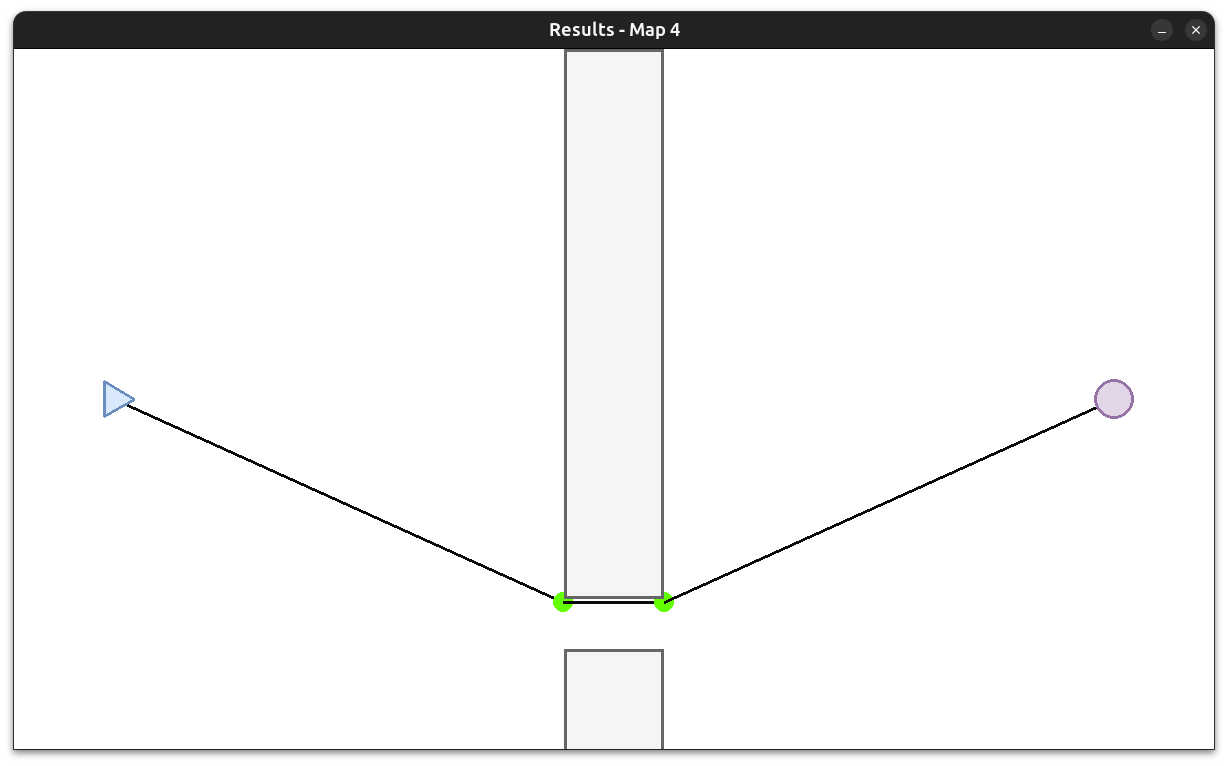
\includegraphics[width=\textwidth]{IMAGES/part3/rmap4.png}
		\caption*{Result for map 4}
		\label{fig:rmap4}
	\end{subfigure}
	\vfill
	\begin{subfigure}[b]{0.24\textwidth}
		\centering
		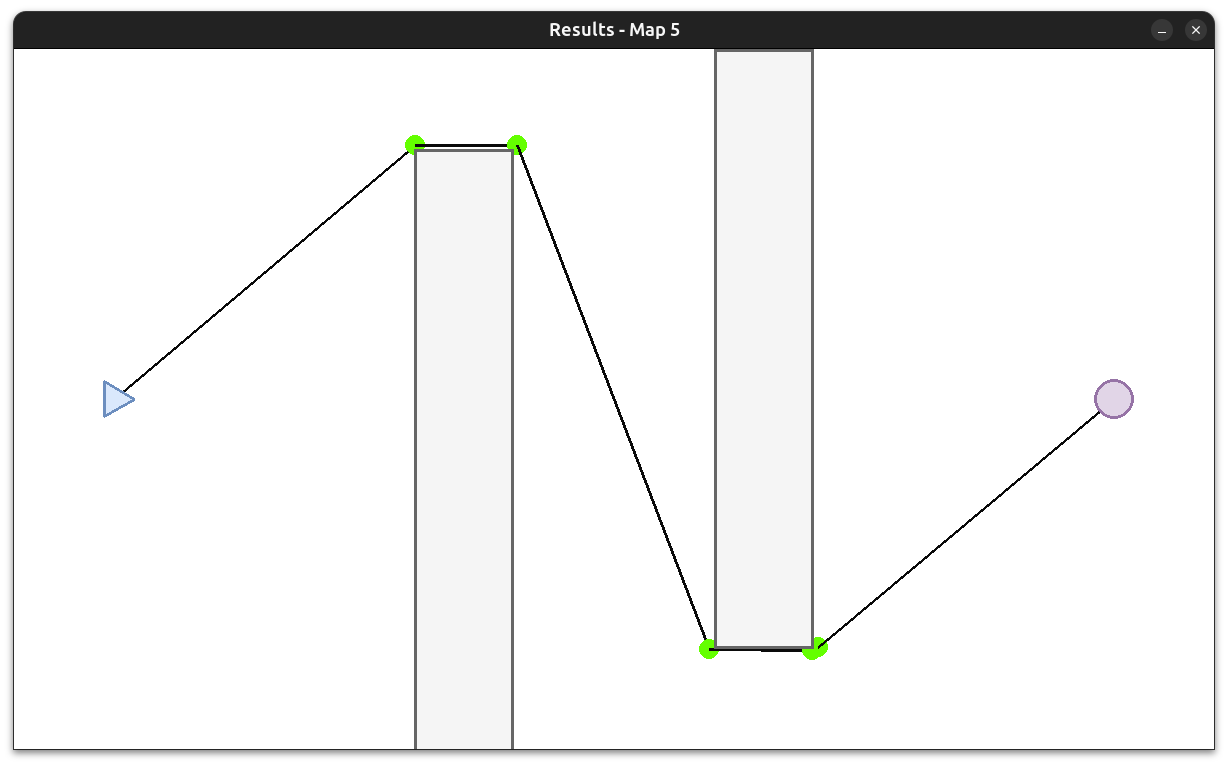
\includegraphics[width=\textwidth]{IMAGES/part3/rmap5.png}
		\caption*{Result for map 5}
		\label{fig:rmap5}
	\end{subfigure}
	\hfill
	\begin{subfigure}[b]{0.24\textwidth}
		\centering
		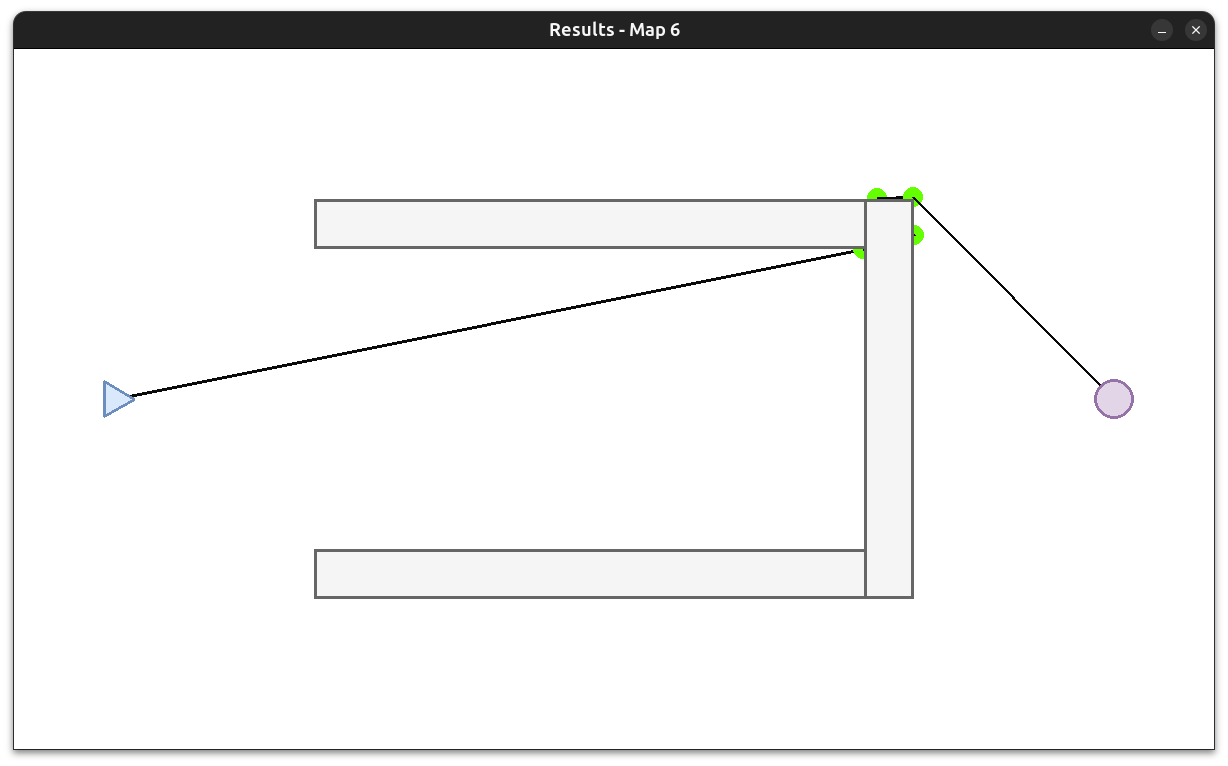
\includegraphics[width=\textwidth]{IMAGES/part3/rmap6.png}
		\caption*{Result for map 6}
		\label{fig:rmap6}
	\end{subfigure}
	\hfill
	\begin{subfigure}[b]{0.24\textwidth}
		\centering
		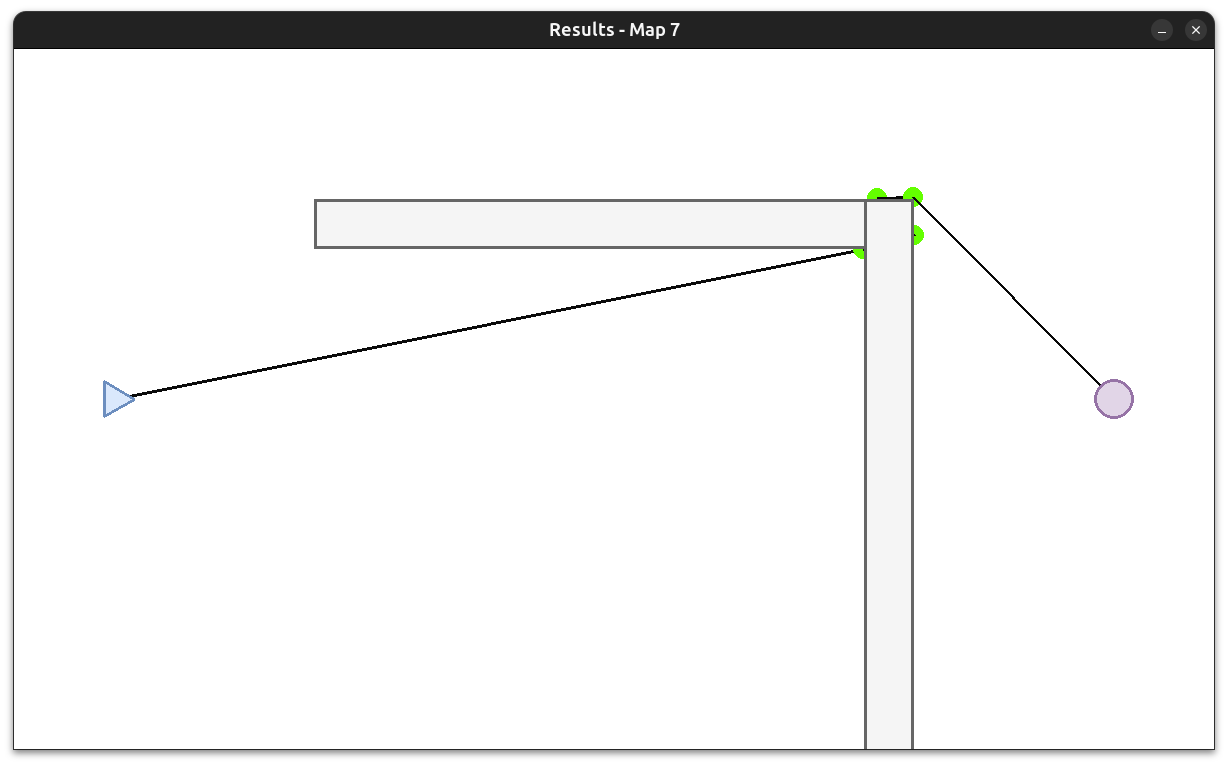
\includegraphics[width=\textwidth]{IMAGES/part3/rmap7.png}
		\caption*{Result for map 7}
		\label{fig:rmap7}
	\end{subfigure}
	\hfill
	\begin{subfigure}[b]{0.24\textwidth}
		\centering
		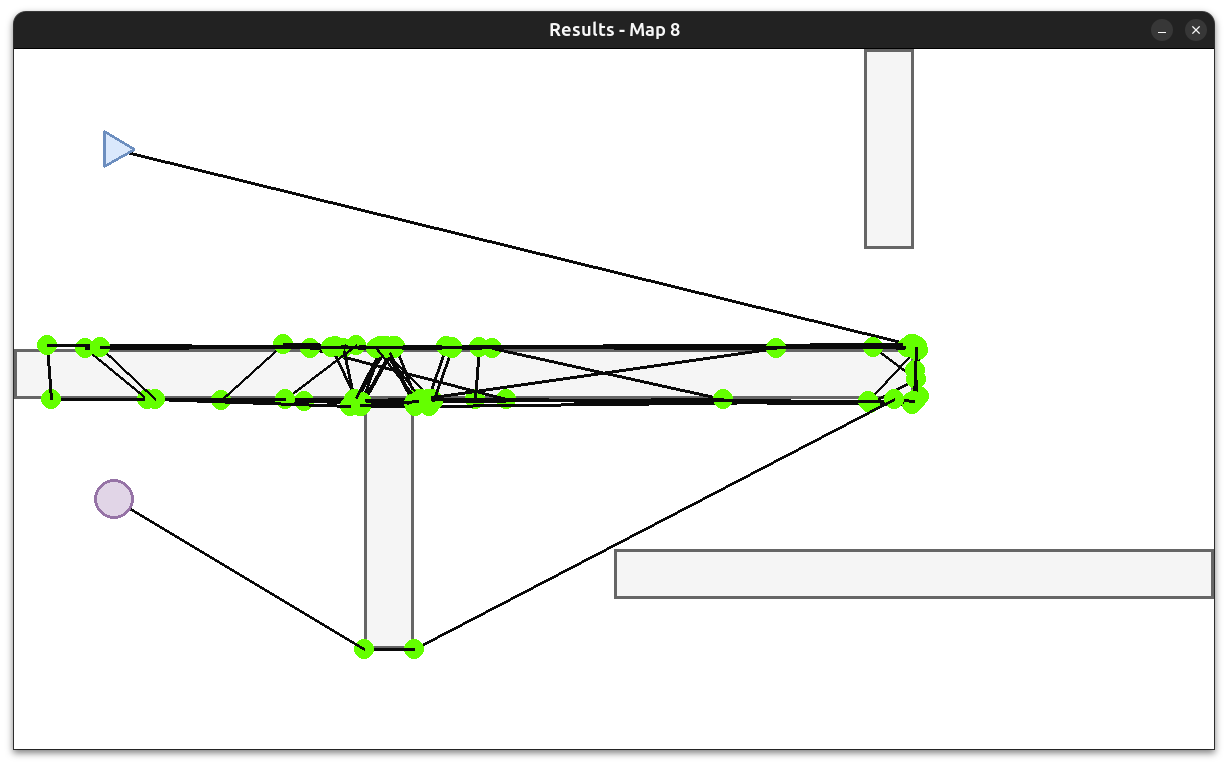
\includegraphics[width=\textwidth]{IMAGES/part3/rmap8.png}
		\caption*{Result for map 8}
		\label{fig:rmap8}
	\end{subfigure}
	\caption{Results on the benchmark maps}
	\label{fig:results_benchmark_maps}
\end{figure}

On maps 6 and 7, the robot is blocked by the angles of the walls. On map 8, although it appears that the robot finds a path, the lines within the wall indicate otherwise. The method is blocked by the wall just before reaching the waypoint. This outcome can be anticipated by examining the shape of the walls near the waypoint. \autoref{fig:fail_explain} illustrates why the new method fails in the situations presented by maps 6, 7, and 8. The numbers represent the iteration at which each point is created, with red numbers indicating the iteration when the method is certain to fail due to the geometry and the way the method is implemented. While this is not tragic, it is important to note that my goal is to explore a cave, and the robot is likely to occur only once and not repeatedly when a part of the map is fully explored. For these cases, I implemented another path planning algorithm introduced in the next secion. 

\begin{figure}[H]
	\centering
	\begin{subfigure}[b]{0.45\textwidth}
		\centering
		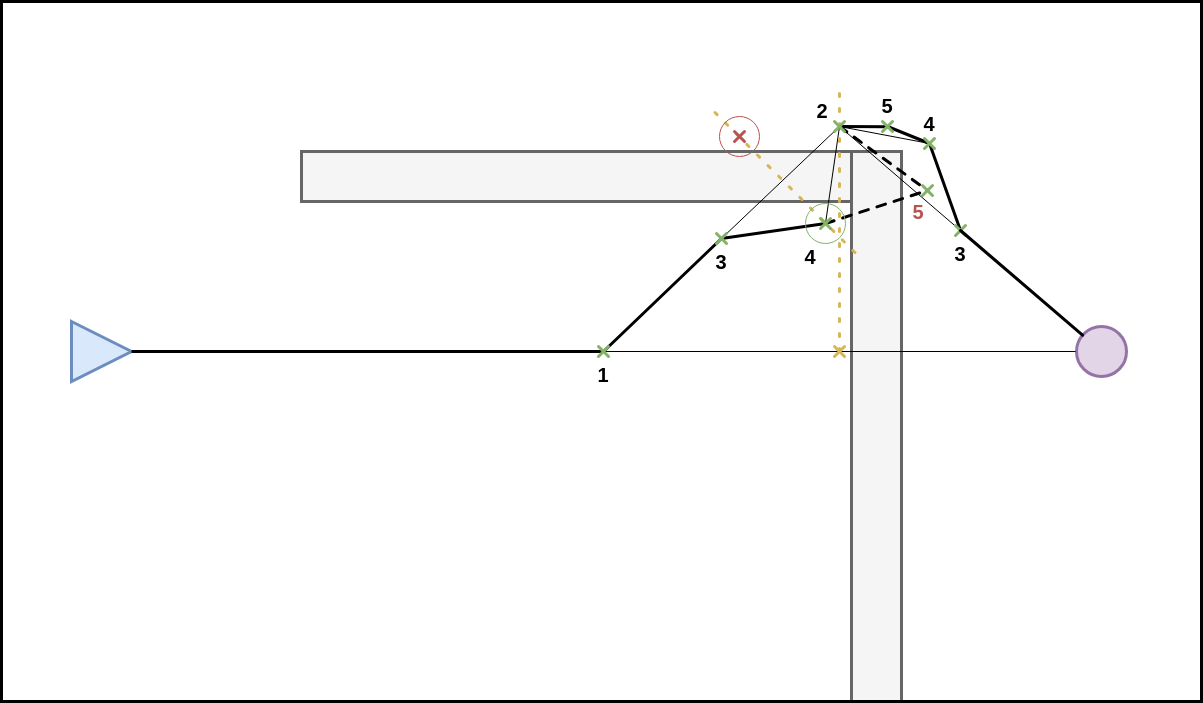
\includegraphics[width=\textwidth]{IMAGES/part3/explain_map7.png}
		\caption{Failure on map 7}
		\label{fig:failure_map7}
	\end{subfigure}
	\hfill
	\begin{subfigure}[b]{0.45\textwidth}
		\centering
		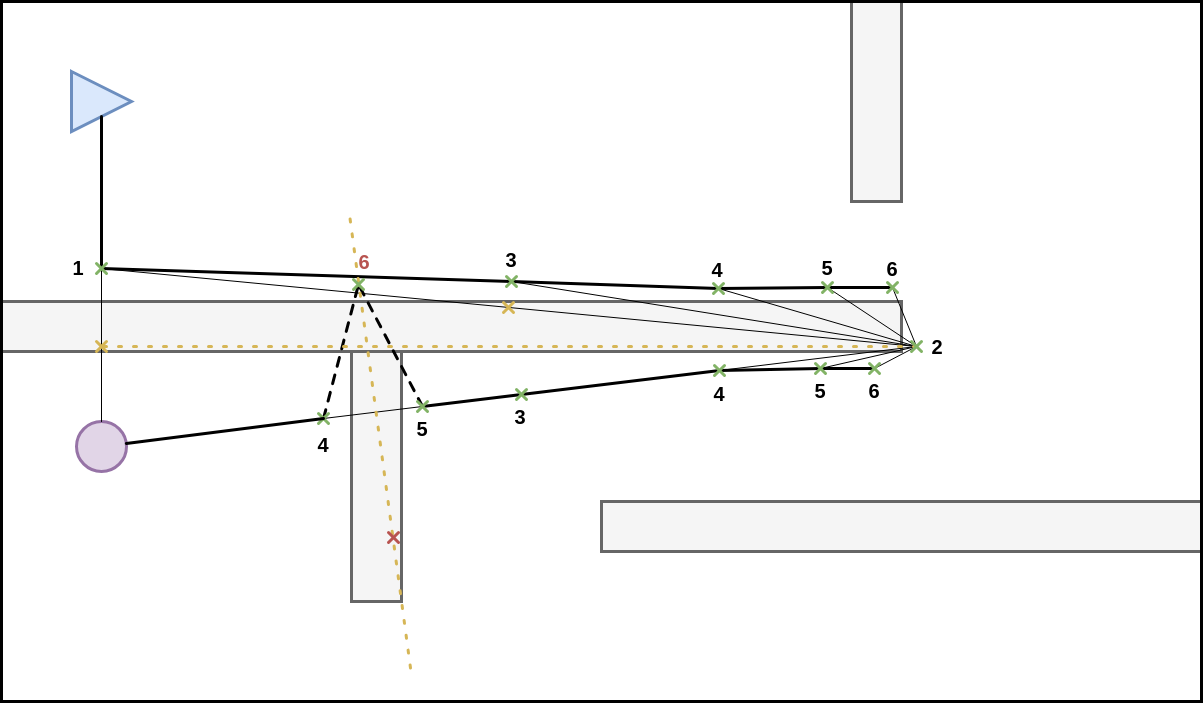
\includegraphics[width=\textwidth]{IMAGES/part3/explain_map8.png}
		\caption{Failure on map 8}
		\label{fig:failure_map8}
	\end{subfigure}
	\caption{Failure explanation for introduced method}
	\label{fig:fail_explain}
\end{figure}


The calculation with the cellular automata is done with the following parameters, the size of the cells are 2 by 2 metric unit (mu) giving a uncertanty of $\pm 2$ mu. The granularity is set to 5 for all cases without circular shape and 20 otherwise.
\tobedone

\textbf{Lenght of the path found in metric unit (mu)}
\begin{table}[H]
	\centering
	\begin{tabular}{c c c c c c}
		\hline
		Map & Theoretically & Method & Relative difference ($\%$) & Cellular Automata ($\pm 2$ mu) & Error ($\%$)\\
		\hline
		Map 1 & 1081 & 1084 & 0.3 &  & \\
		Map 2 & 1121 & 1125 & 0.4 & 1122 & 0.1\\
		Map 3 & 1122 & 1125 & 0.4 & 1122 & 0\\
		Map 4 & 1084 & 1088 & 0.4 & 1086 & 0.2\\
		Map 5 & 1521 & 1531 & 0.7 & 1522 & 0.1\\
		Map 6 & 1166 & - &  & 1168 & 0.2\\
		Map 7 & 1166 & - &  & 1168 & 0.2\\
		Map 8 & 1776 & - &  &  & \\
		\hline
	\end{tabular}
	\caption{Benchmark results for the new method}
	\label{tab:benchmark_results}
\end{table}

The \autoref{tab:benchmark_results} gives us the relative difference between the method introduced and the theoretical value for the shortest path. As we can see the path when found is always under $1\%$ longer than the shortest one, moreover, we can imagine less to $1\%$ if the compute precisly the point on the border, due to the iterative process, the point can be place up to a distance of zero to the step we move the point to check if it is safe.

Moreover, the lattice approach for finding the shortest algorith is very good in this benchmark, within the range of uncertancy, the algorith always found the shortest path distance.


\subsection{Dijkstra's algorithm}

The second algorithm for path planning uses Dijkstra's method. The goal is to navigate to the nearest point of the map where a robot already passed to the waypoint. The waypoints are located on the frontiers of the robot's explored area, calculated using lidar data. This ensures that the path from the nearest location to the waypoint is a straight line free from obstacles. 

Dijkstra's algorithm is an algorithm to find the shortest path from a source to a final node in a weighted graph.\cite{dijkstra_1959}. It works by iteratively selecting the node with the smallest tentative distance, updating the distances to its neighbors, and marking it as visited. This process continues until all nodes have been visited or the shortest path to the target node is determined.\cite{dijkstra_anim_wiki_2025}

To ensure the path to the nearest point exists, the robot will move only on cells previously traversed by a robot. This path will be shortened by the algorithm described earlier.
If the robot remains in a certain area for too long, indicating a deadlock, the Dijkstra path is computed to guide the robot out. This emergency path is only calculated when the robot is in a deadlock.

\textbf{Perfomances}

On an AMD Ryzen™ 5 3500U, using \textit{Python} and the map in \autoref{fig:real_map_40}, the robot computes the next global path in an average of $1.02 \times 10^{-1}$ seconds, approximately 98 times per second. This performance is suitable for real-time navigation and obstacle avoidance.

In the simulator, to be more computationally friendly, I simplified the method during implementation by computing only the next point. The difference in trajectory can be seen in \autoref{fig:traj_diff_maps}. This approach sacrifices the optimal path for reduced computational time. The difference in path can be significant, as shown in \autoref{fig:traj_diff_map5}. The path with the blue-green dots can illustrate how the robot navigates without prior knowledge of its environment before reaching the target point.

\begin{figure}[H]
	\centering
	\begin{subfigure}[b]{0.45\textwidth}
		\centering
		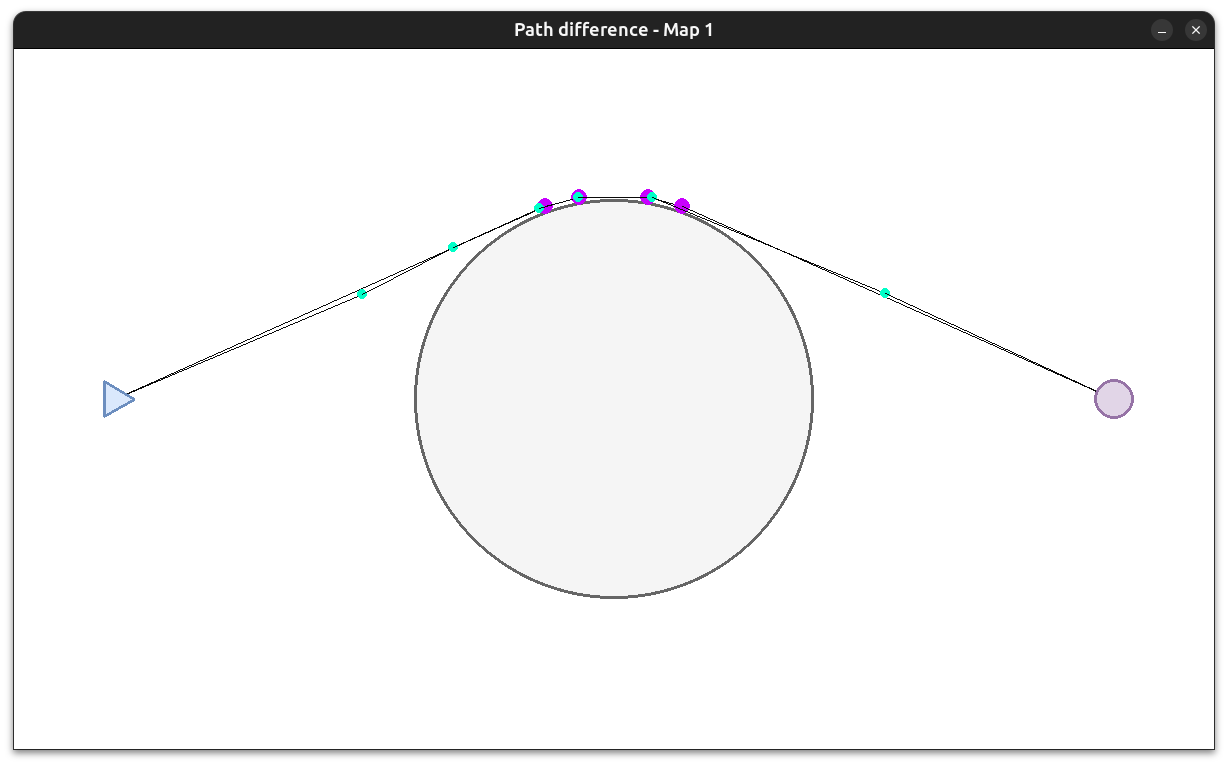
\includegraphics[width=\textwidth]{IMAGES/part3/traj_diff_map1.png}
		\caption{Trajectory difference on map 1}
		\label{fig:traj_diff_map1}
	\end{subfigure}
	\hfill
	\begin{subfigure}[b]{0.45\textwidth}
		\centering
		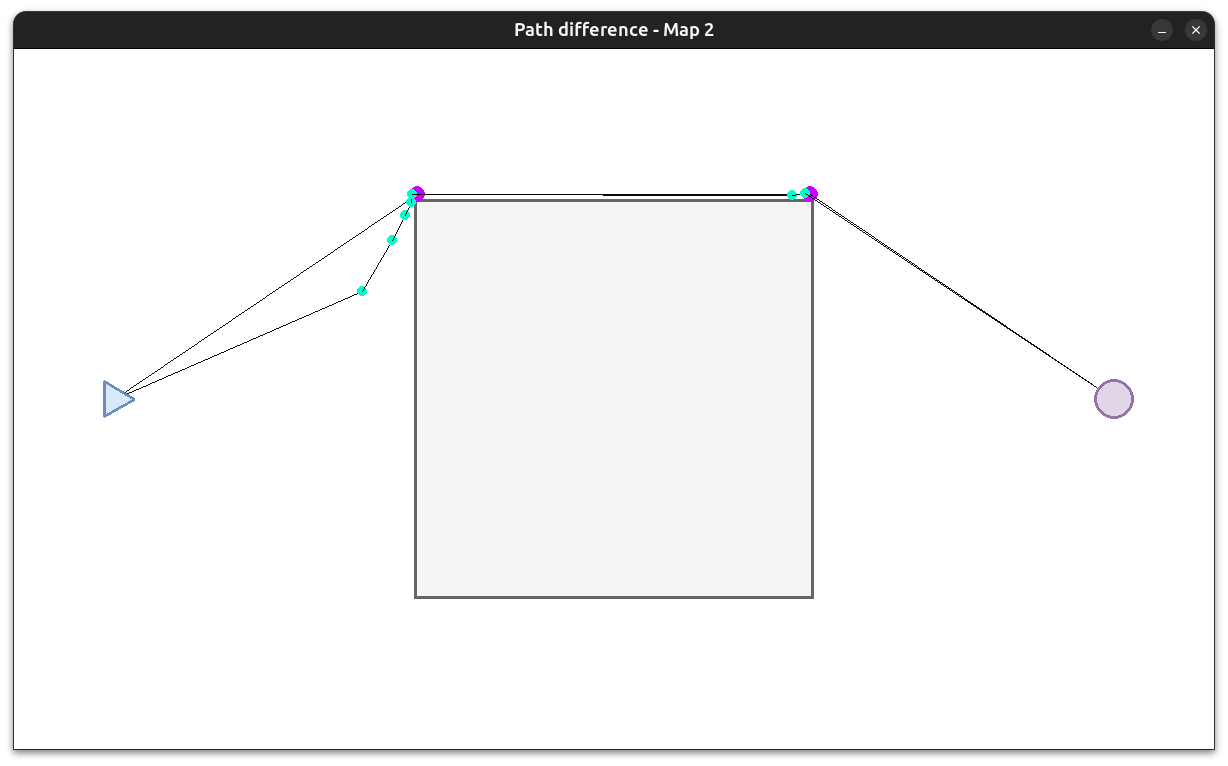
\includegraphics[width=\textwidth]{IMAGES/part3/traj_diff_map2.png}
		\caption{Trajectory difference on map 2}
		\label{fig:traj_diff_map2}
	\end{subfigure}
	\vfill
	\begin{subfigure}[b]{0.45\textwidth}
		\centering
		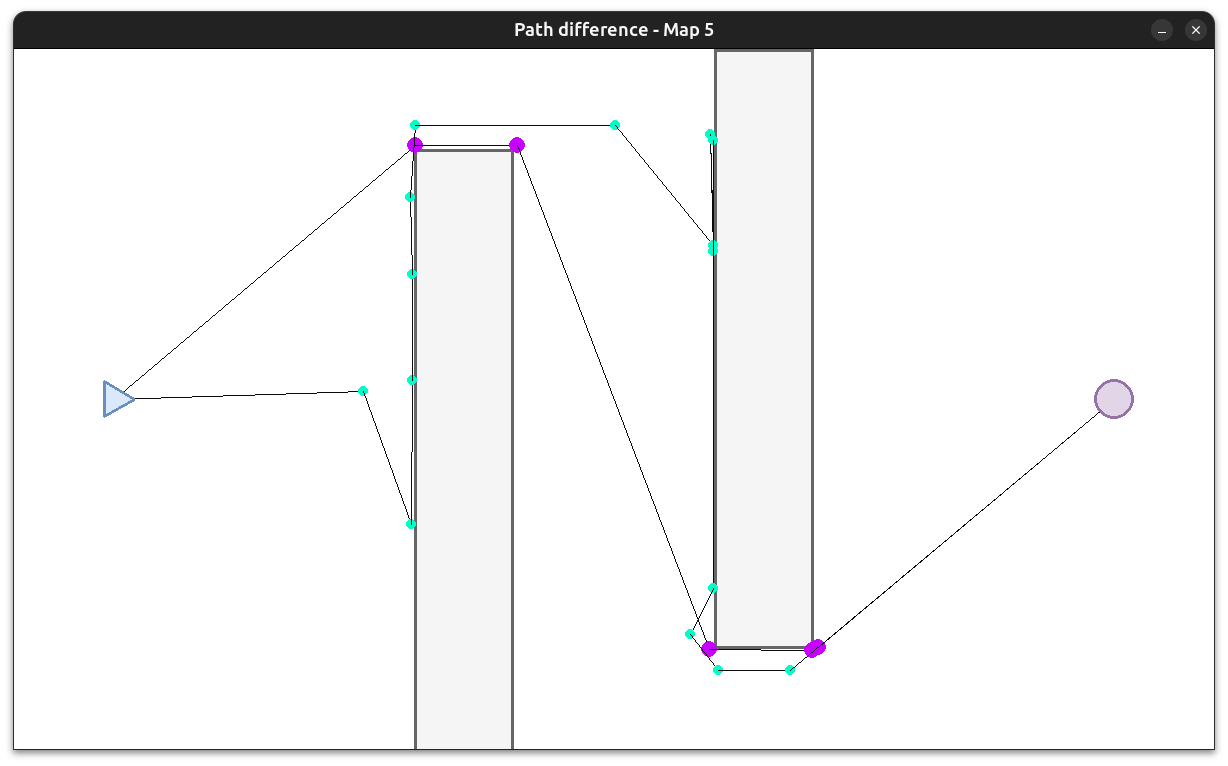
\includegraphics[width=\textwidth]{IMAGES/part3/traj_diff_map5.png}
		\caption{Trajectory difference on map 5}
		\label{fig:traj_diff_map5}
	\end{subfigure}
	\caption{Trajectory differences on maps 1, 2, and 5}
	\label{fig:traj_diff_maps}
\end{figure}

On the same map and laptop, the local approach for path planning is significantly more efficient in terms of computational time. The average computation time is $8.20 \times 10^{-4}$ seconds, allowing for approximately 1220 executions per second. Despite the method's poor performance in the benchmark, it performs well in the simulator, resulting in better map exploration and improved path quality. The \autoref{fig:map_exploration_comparison} shows the two maps after exploration of only one robot.

\begin{figure}[H]
	\centering
	\begin{subfigure}[b]{0.45\textwidth}
		\centering
		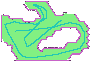
\includegraphics[width=\textwidth]{IMAGES/part3/map_explored_using_gwp.png}
		\caption{Map explored using global waypoint path}
		\label{fig:map_explored_using_gwp}
	\end{subfigure}
	\hfill
	\begin{subfigure}[b]{0.45\textwidth}
		\centering
		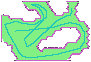
\includegraphics[width=\textwidth]{IMAGES/part3/map_explored_using_lwp.png}
		\caption{Map explored using local waypoint path}
		\label{fig:map_explored_using_lwp}
	\end{subfigure}
	\caption{Comparison of map exploration using global and local waypoint paths}
	\label{fig:map_exploration_comparison}
\end{figure}


\subsection{Performance Analysis Methodology}

To evaluate the performance of the algorithm, we will use the following criteria: range, robustness, and completeness. These criteria are part of a broader methodology that also includes effectiveness and speed.

\subsubsection{Delimited Range of Application}
The combination of the two algorithms is well-suited for both open spaces and medium-sized cavities. However, the method performs significantly better in open spaces, as suggested by the benchmark results. This approach could be considered for aeronautical applications. It should be noted that in narrow cavities, Dijkstra's algorithm is likely to be executed each time a new direction is chosen.

\subsubsection{Robustness to Failure and Uncertainty}
Robustness to failure and uncertainty means that the robot must handle all possible cases, such as being in a deadlock and failing to exit it. The second part of the method, Dijkstra's algorithm, ensures that the robot can exit any situation by moving back along its path.

\subsubsection{Completeness}
Completeness means that the robot must explore all the domain possible to be explored or accomplish all the possible tasks given to it. To study completeness, a vast range of tests must be conducted. At this stage of the study, it is not certain that the algorithm is complete.

\subsection{Global waypoint computing}

Now the local navigation is set, we need to define how to select the next waypoint occording to the map. First of all this is done by computing the frontiers of the know domains using image detection method.


To extract the open frontiers of the map, I propose the following method:
\begin{enumerate}
	\item Obtain the live grid map of the environment.
	\item Generate a thresholded version of the map to distinguish wall areas from other regions (unknown and free spaces).
	\item Identify the contours of the map by appliying an Adaptive Gaussian Treshold.
	\item Apply a single iteration of dilation on the wall treshold.
	\item Add the contour map from the dilated wall image to isolate the open frontiers.
\end{enumerate}

The \autoref{fig:open_frontiers} shows an example of the method described above on the \autoref{fig:map_open_frontiers}

\begin{figure}[H]
	\centering
	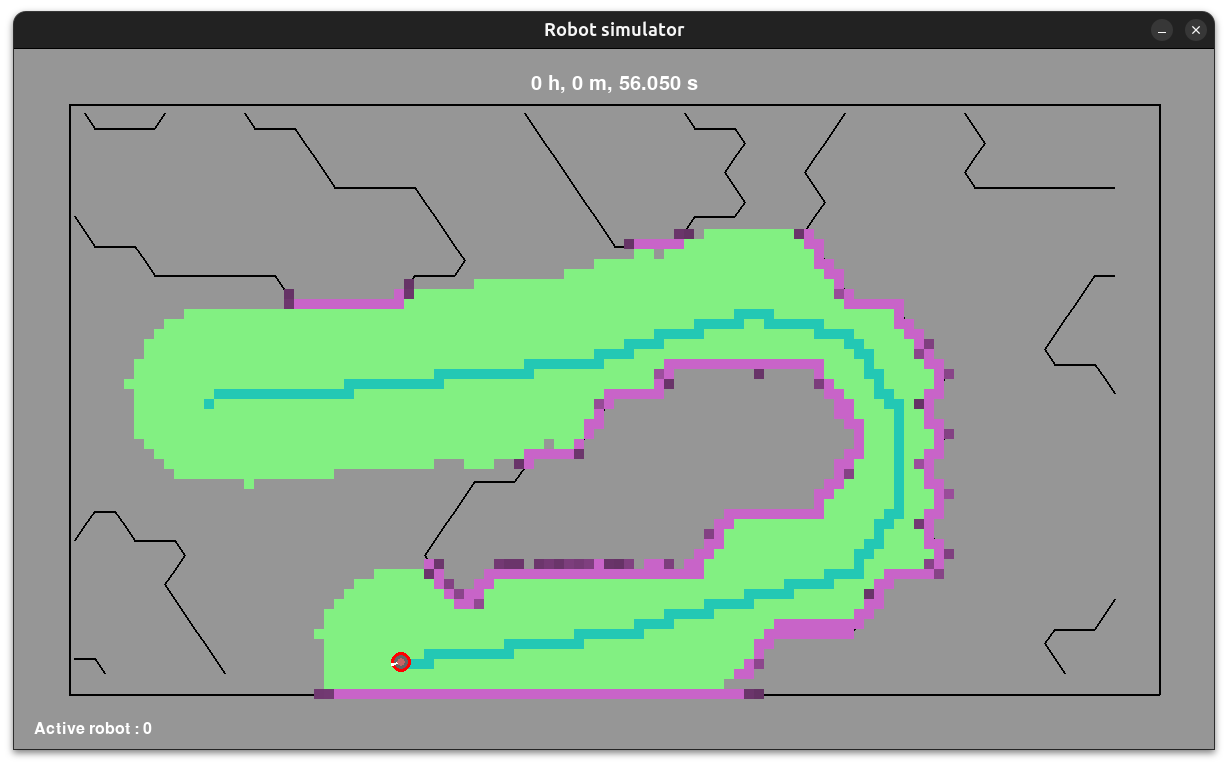
\includegraphics[width=0.6\textwidth]{IMAGES/part3/map_open_frontiers.png}
	\caption{Open frontiers of the map example}
	\label{fig:map_open_frontiers}
\end{figure}

\begin{figure}[H]
	\centering
	\begin{subfigure}[b]{0.45\textwidth}
		\centering
		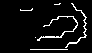
\includegraphics[width=\textwidth]{IMAGES/part3/treshold_image.png}
		\caption{Thresholded version of the live grid map}
		\label{fig:subfigure1}
	\end{subfigure}
	\hfill
	\begin{subfigure}[b]{0.45\textwidth}
		\centering
		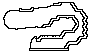
\includegraphics[width=\textwidth]{IMAGES/part3/adaptative_treshold.png}
		\caption{Adaptative thresholded version of the map}
		\label{fig:subfigure2}
	\end{subfigure}
	\vfill
	\begin{subfigure}[b]{0.45\textwidth}
		\centering
		
\includegraphics[width=\textwidth]{IMAGES/part3/dilatation_image.png}
		\caption{Dilatation of the wall thresholded map}
		\label{fig:subfigure3}
	\end{subfigure}
	\hfill
	\begin{subfigure}[b]{0.45\textwidth}
		\centering
		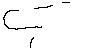
\includegraphics[width=\textwidth]{IMAGES/part3/sum_image.png}
		\caption{Sum of the (b) and (c) images highlighting open frontiers}
		\label{fig:subfigure4}
	\end{subfigure}
	\caption{Steps to extract the open frontiers from the live grid map}
	\label{fig:open_frontiers}
\end{figure}

Once all frontiers are computed, an algorithm assigns a weight to each cell, and the robot selects the cell with the minimal weight. \autoref{fig:weighted_frontiers} shows the weights, with only one out of every ten points displayed for clarity.

\begin{figure}[H]
	\centering
	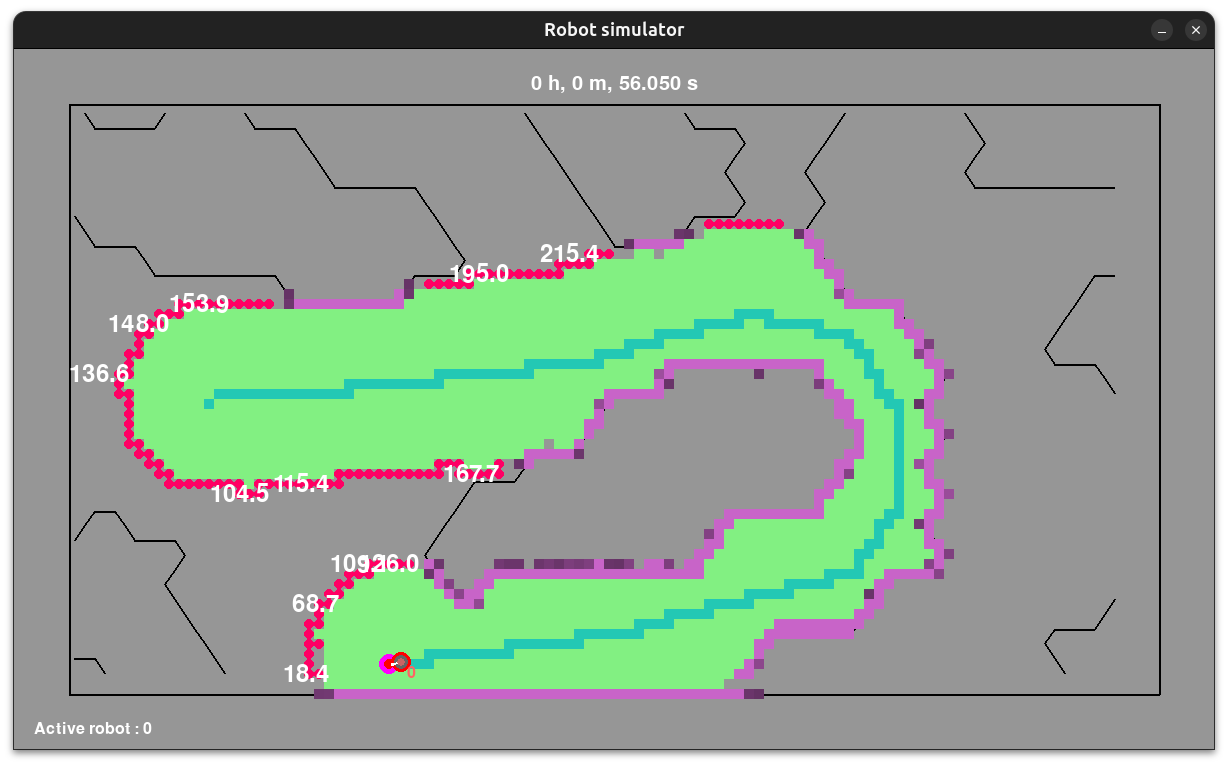
\includegraphics[width=0.6\textwidth]{IMAGES/part3/weighted_fontiers.png}
	\caption{Weighted frontiers of the map}
	\label{fig:weighted_frontiers}
\end{figure}

The weights are calculated using four parameters of the robot: its position, heading, speed, and angular speed. Each of these parameters is assigned a different weight to prioritize one constraint over the others, such as position, heading, speed, or angular speed.

\end{document}

